\documentclass[SE,lsstdraft,authoryear,toc]{lsstdoc}
% GENERATED FILE -- edit this in the Makefile
\newcommand{\lsstDocType}{SITCOMTN}
\newcommand{\lsstDocNum}{154}
\newcommand{\vcsRevision}{362d79f-dirty}
\newcommand{\vcsDate}{2025-06-20}


% Package imports go here.
\usepackage{xcolor}
\usepackage{hyperref}
\usepackage{fancyvrb}

% Local commands go here.

% red, green, blue, cyan, magenta, yellow, black, gray, white, darkgray, lightgray, brown, lime, olive, orange, pink, purple, teal, violet
% % personal tags should probably have argument for date
\newcommand{\PersonalTag}[3]{{\color{#2}{{\bf #1} #3}}}
% choose a color for yourself from the xcolor table here: https://www.overleaf.com/learn/latex/Using_colours_in_LaTeX
\newcommand{\any}[1]{\PersonalTag{}{red}{#1}}
\newcommand{\eac}[1]{\PersonalTag{Eric}{purple}{#1}}
\newcommand{\needcite}[1]{{\color{red} citation needed {#1}}\xspace}
\newcommand{\codetodo}[1]{{\color{gray} [code TODO: {#1}]}\xspace}
\newcommand{\halp}[2]{\textbf{\color{blue} INSTRUCTIONS FOR CONTRIBUTORS ({#1}): {#2}}\xspace}

%If you want glossaries
%\input{aglossary.tex}
%\makeglossaries

\title{Initial studies of photometric redshifts for ComCam data}

% This can write metadata into the PDF.
% Update keywords and author information as necessary.
\hypersetup{
    pdftitle={Photometric redshifts for ComCam data},
    pdfauthor={Melissa Graham},    
    pdfkeywords={}
}

% Optional subtitle
% \setDocSubtitle{A subtitle}

\author{%
  Eric Charles,
  John Franklin Crenshaw,
  Tianqing Zhang, 
  Sam Schmidt,
  Prakruth Adari, 
  Melissa Graham,  
}

\setDocRef{SITCOMTN-154}
\setDocUpstreamLocation{\url{https://github.com/lsst-sitcom/sitcomtn-154}}

\date{\vcsDate}

% Optional: name of the document's curator
% \setDocCurator{The Curator of this Document}

\setDocAbstract{%
This technote holds reports based on the first analyses of the Data Preview 1 (DP1) ComCam data by the Science Unit for photometric redshifts.  The Science Unit developed training and test datasets by matching DP1 data to high-quality reference redshifts obtained with spectroscopy, Grism data, and multi-band photometry.  
The Science Unit then used the RAIL software package to make photometric redshifts estimates using eight different algorithms, developed simple scientific performance metrics, used those metrics to explore how the performance of the algorithms varied with configuration changes, derived more optimized configurations of the algorithms and tested the performance of those configurations.   
}

% Change history defined here.
% Order: oldest first.
% Fields: VERSION, DATE, DESCRIPTION, OWNER NAME.
% See LPM-51 for version number policy.
\setDocChangeRecord{%
  \addtohist{1}{YYYY-MM-DD}{Unreleased.}{Melissa Graham}
}


\begin{document}

% Create the title page.
\maketitle
% Frequently for a technote we do not want a title page  uncomment this to remove the title page and changelog.
% use \mkshorttitle to remove the extra pages

% ADD CONTENT HERE
% You can also use the \input command to include several content files.
\section{Introduction}
\label{sec:intro:0}

The Vera C. Rubin Observatory’s Data Preview 1 (DP1) marks an important milestone in preparing for the forthcoming Legacy Survey of Space and Time (LSST), offering a valuable opportunity to test and validate scientific tools and workflows on precursor imaging data~\citep{RTN:095}. Among the core scientific objectives of LSST is the estimation of photometric redshifts (\photozs) for billions of galaxies, enabling extragalactic astrophysics and cosmological analyses that rely on redshift estimates and distributions.  Accordingly, the Rubin project developed a roadmap to providing high-quality \photozs for the scientific community~\citep{DMTN:049}.

Although \photoz are not a DP1 deliverable, the ``Photo-z Science Unit'' was asked to generate \photoz estimates for every galaxy in DP1 using the available multi-band imaging on a best-effort basis, laying the groundwork for future large-scale applications.  This effort required integrating realistic data processing with scalable machine learning techniques capable of delivering precise redshift predictions across varied galaxy populations.

To accomplish this task, we employed the RAIL (Redshift Assessment Infrastructure Layers) software package, a flexible and modular platform designed for \photoz estimation and evaluation\citep{RAIL}.  Specifically, we used RAIL to train \photoz estimation algorithms on high-quality redshift training sets cross-matched to the DP1 photometric catalog.  

This note describes the resulting best-effort \photoz catalogs, which should be regarded as extremely preliminary, and the tools used and the steps taken to generate those catalogs.  In addition, we describe relevant features of the DP1 photometric data, the spectroscopic calibration datasets and the resulting \photoz catalogs.   Additional details about data products and data distribution are included as appendices.

We expect feedback from science users as they explore the data and discover issues that we have not anticipated, and that we will incorporate that feedback in future work.

\section{Data}
\label{sec:data:0}

\subsection{Rubin DP1}
\label{sec:data:dp1}

The Rubin Observatory’s Data Preview 1 (DP1) dataset is the first public release of Rubin observatory imaging data processed through the LSST Science Pipelines, serving as a critical testbed for scientific and technical validation ahead of full LSST operations.  DP1 is based on observations from the LSST commissioning camera (LSSTComCam) and includes multi-band optical imaging in u, g, r, i, z and y filters over several square degrees of sky.  The dataset consists of processed images, source catalogs, and associated metadata, all formatted using the Rubin Data Butler system in the same way as full LSST data products.  Although smaller in scale than future LSST datasets, DP1 offers realistic photometric measurements, object detection, and data structures, making it an invaluable resource for developing and testing algorithms for tasks such as \photoz estimation, object classification, and data quality assessment.

Critially, the fields selected for ComCam observation included the Extended Chandra Deep Field South (ECDFS), for which many high-quailty redshifts exist from other surveys. 


\subsubsection{Preparation of photometric object catalogs}
\label{sec:data:dp1:preparation}

The Rubin Data Management (Rubin DM) pipeline measures multiple types of object photometry, the first stage in creating a \photoz catalog was to determine which measured photometry we would use as inputs.  In this note, we generally use the 1.0 arc-second Gaussian Aperture fluxes and their associated errors, e.~g.~\texttt{u\_gaap1p0Flux} and \texttt{u\_gaap1p0FluxErr}.  These fluxes should provide good measures of consistent galaxy colors within the defined aperture, ideal for \photoz estimation, though they may not necessarily reflect the colors of the overall galaxy if there is a significant color gradient and the galaxy is larger than the 1.0 arc-second aperture.  This choice of photometric measurement may not be ideal, and investigation into the optimized set of photometric inputs will continue into the future.   The only exceptions to this are that we used \texttt{i\_psfFlux} in the initial broad data cuts, and that we briefly explored several of the other fluxes as part of the initial validation of our \photoz analysis pipelines. 

Preparing object catalog data for \photoz algorithm training and estimation included five steps:

\begin{enumerate}
\item{Applying quality cuts to the object catalog.   We developed selections for the training and test datasets (\selection{match\_xxx}), and two additional selections for full DP1 catalogs: one applicable for fields with observations in only four bands (\selection{gold\_4\_band}), the other for fields with observations in all six bands (\selection{gold}).  These selections are described below.}
\item{Converting fluxes in nJy to AB magnitudes ($m_\text{AB} = -2.5 \log_{10}(f_\nu / \text{nJy}) + 31.4$)}
\item{De-reddening to account for Galactic dust.  We use the SFD dust maps\citep{SFD}.}
\item{Cross-matching objects with reference catalogs that include redshift information as described in Sec.~\ref{sec:data:reference}.}
\item{Shuffling and splitting the resulting catalog into \dataset{training} and \dataset{test} data sets.}
\end{enumerate}

The data selection criteria that we used were:
\begin{itemize}
\item{\selection{match\_prelim}: first version of matching to high-quality redshift catalogs in the ECDFS field,  see Sec.~\ref{sec:data:reference}.}
\item{\selection{match\_ecdfs}: updated matching to high-quality redshift datalogs in the ECDFS field, see Sec.~\ref{sec:data:reference}.}
\item{\selection{match\_desi}: matching to DESI redshift catalogs in the \field{Rubin SV 38 7} field, see Sec.~\ref{sec:data:desi}.}
\item{\selection{gold}: \code{Detection in 'ugrizy'  \&\& i\_psfFlux / i\_psfFluxErr > 5 \&\& ( g\_extendedness > 0.5 || r\_extendedness > 0.5)}.}
\item{\selection{gold\_4\_band}: \code{Detection in 'griz' \&\& i\_psfFlux / i\_psfFluxErr > 5 \&\& ( g\_extendedness > 0.5 || r\_extendedness > 0.5)}.}
\end{itemize}

To create the \dataset{training} and \dataset{test} data sets, we followed steps 1--5, while for the larger unlabeled data sets we followed steps 1--3.  Specifically, for DP1, the \field{ECDFS}, \dataset{EDFS} and \dataset{Rubin SV 95 -25} fields have observation in 6 bands, and we applied the \selection{gold} target selection.   In \field{Rubin SV 38 7}, DP1 only has observation in 4 bands (``griz''), therefore we applied the \selection{gold\_4\_band} target selection to that field. 


All of these datasets are summarized in Tab.~\ref{tab:dataset}.

\begin{table*}
\centering
\begin{tabular}{lll}
 \hline
    Data set & Selection & Number of objects\\
 \hline
 \hline
  DP1 & None & 2,299,757 \\
 ECDFS+EDFS+SV\_95 & \selection{gold} & 375,610\\
 SV\_38 & \selection{gold\_4\_band} & 169,034\\
 training\_v1 & \selection{match\_prelim}  & 7,000\\
 test\_v1 & \selection{match\_prelim}  & 2,437 \\
 training\_v2 & \selection{match\_ecdfs}  & 4,803\\
 test\_v2 & \selection{match\_ecdfs}  & 1,201 \\
 test\_DESI & \selection{match\_desi}  & 2,728 \\
 \hline
\end{tabular}
\caption{ Summary of the datasets used in this work.  Note that to train models on four-band photometry, we used the same training and test sets as for six-band photometry, but configured the algorithms only to use the 'griz' bands.}
\label{tab:dataset}
\end{table*}



\subsubsection{Data properties}
\label{sec:data:dp1:properties}

We have developed tools to generate diagnostic plots of both the input object catalogs and the \photoz estimates as part of our data analysis.
Fig.~\ref{fig:dp_mags} shows histograms of the AB magnitudes in 1.0 arc-second apertures of objects in the \dataset{test\_v1} dataset, which includes an explicit magnitude cut, $m_{i} < 26.0$.
Fig.~\ref{fig:dp_mag_i_v_redshift} shows the correlation between magnitude and redshift for all objects in the \dataset{test\_v1} data set.  
Fig.~\ref{fig:dp_color_v_redshift} shows the ``adjacent band colors'', i.e., $u-g$, $g-r$, $r-i$, $i-z$, $z-y$ versus redshift for the same, with a series of SED templates (as used by template-fitting algorithms, see Sec.~\ref{sec:method:template}) overlaid.  
Finally, Fig.~\ref{fig:dp_color_v_color} shows the color-color correlations for the same.  In all cases, the 1.0 arc-second aperture magnitudes are used for plotting.

\begin{figure*}
    \centering
    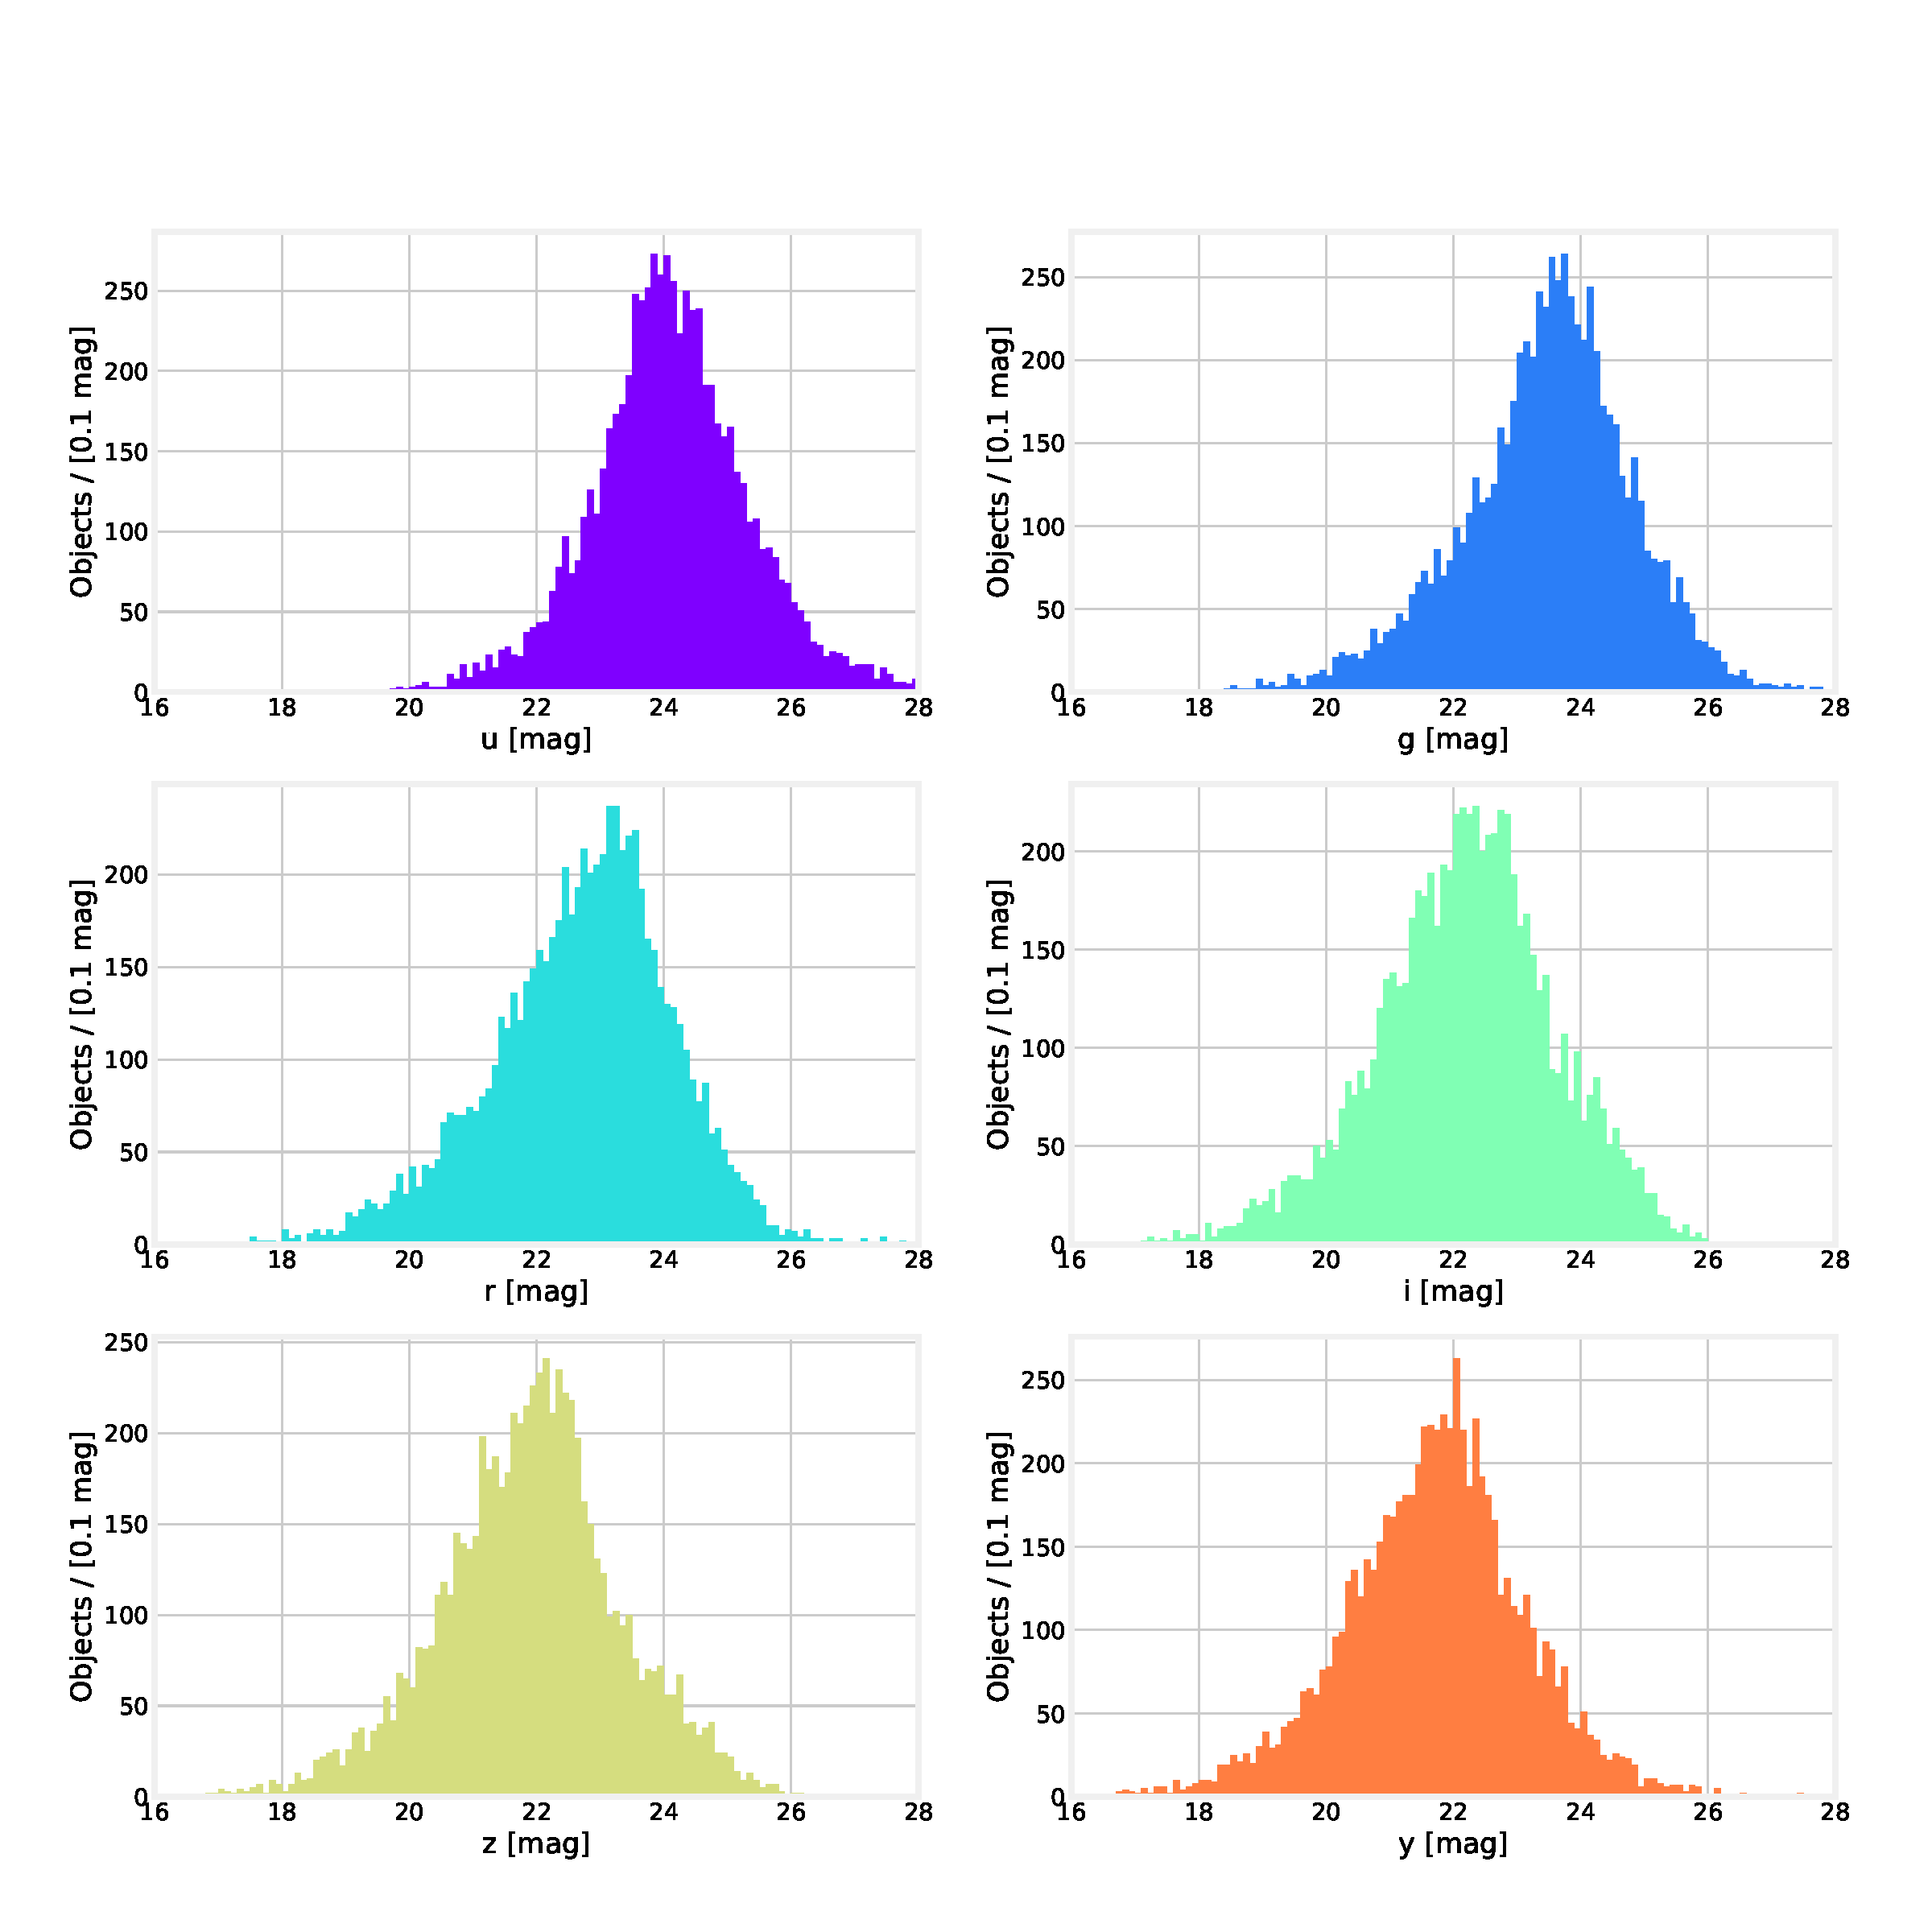
\includegraphics[width=\linewidth]{figures/mags.pdf}
    \caption{1.0 arc-second Gaussian Aperture (Gaap) magnitudes (in AB system) of objects in each of the six Rubin filter bands in the \dataset{test\_v1} dataset.  These aperture magnitudes were used as the inputs for the \photoz algorithms.}
    \label{fig:dp_mags}
\end{figure*}

\begin{figure*}
    \centering
    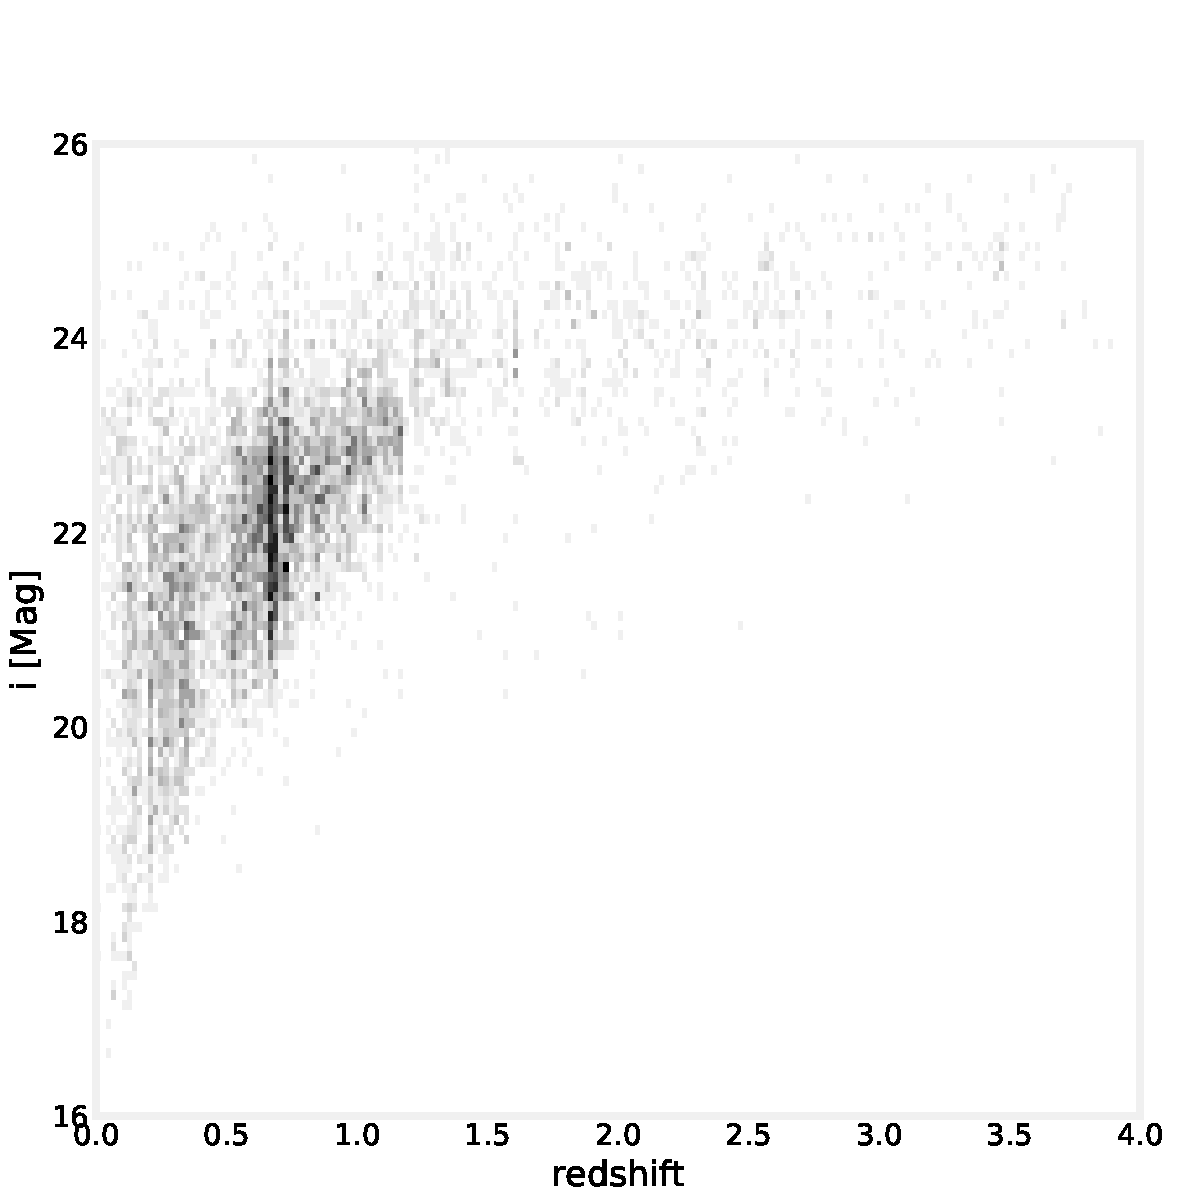
\includegraphics[width=\linewidth]{figures/mag_i_v_redshift.pdf}
    \caption{1.0 arc-second Gaussian Aperture (Gaap) i-band magnitude versus redshift for all objects in the \dataset{test\_v1} dataset.}
    \label{fig:dp_mag_i_v_redshift}
\end{figure*}

\begin{figure*}
    \centering
    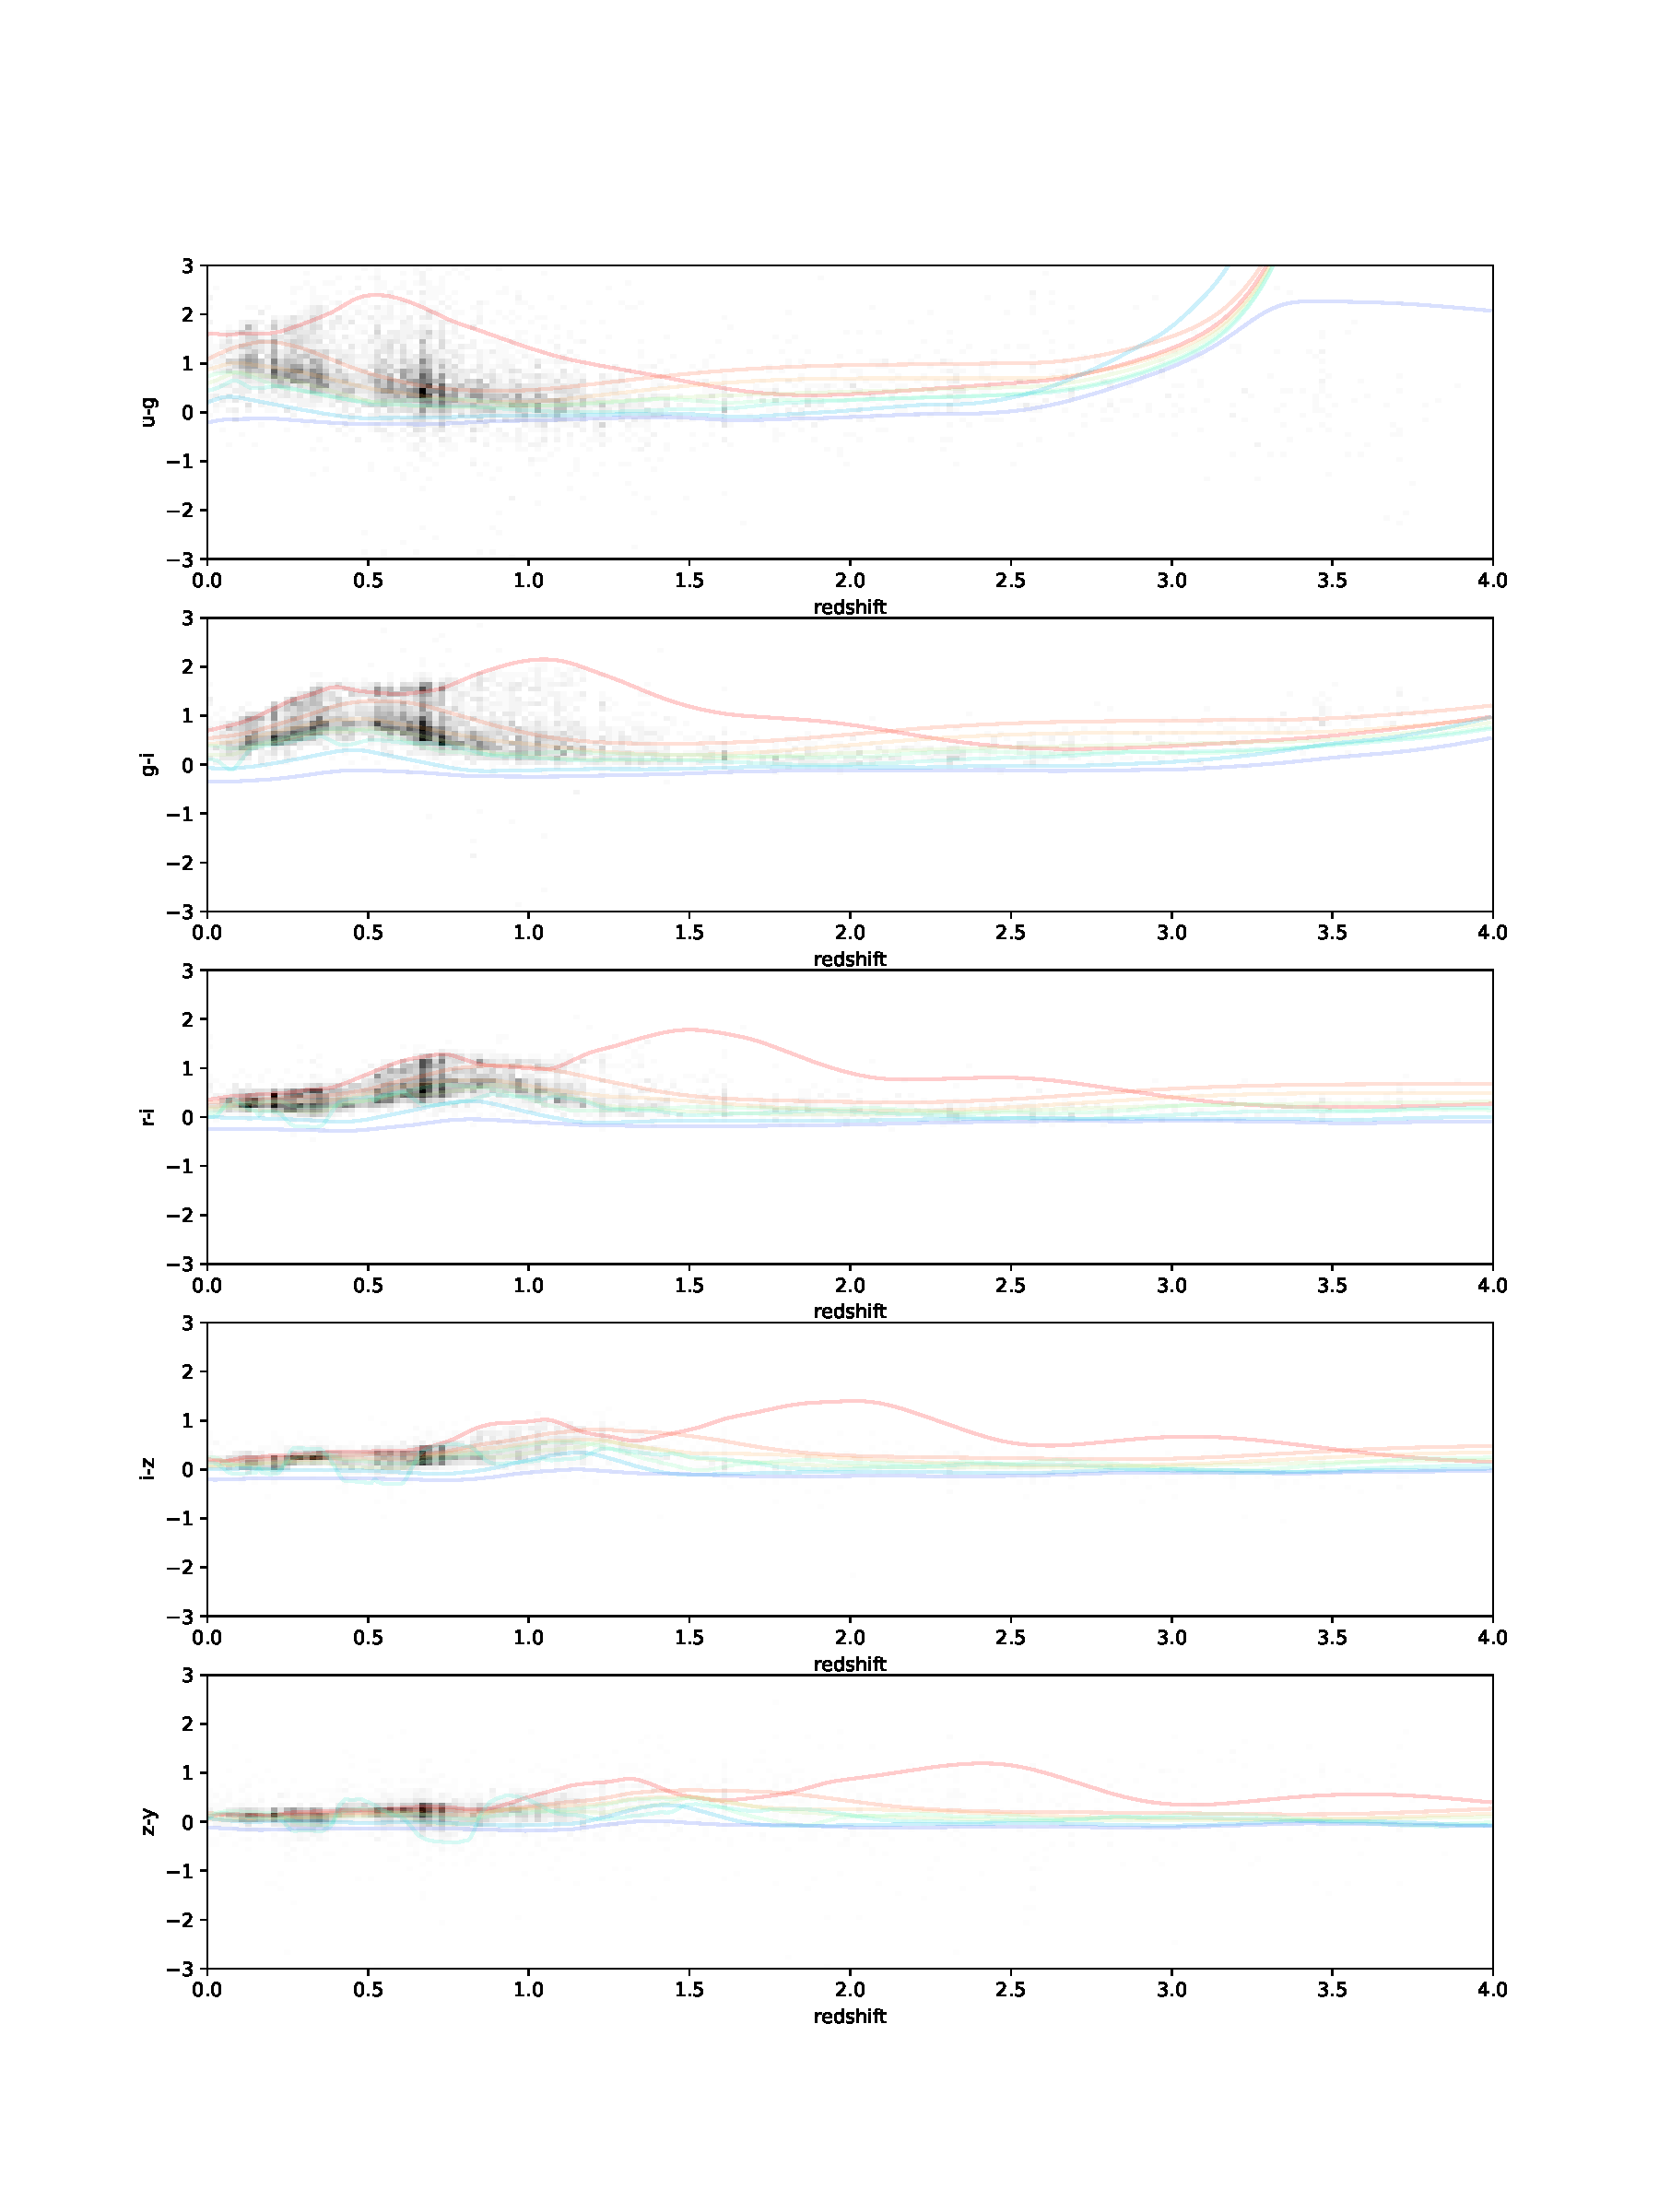
\includegraphics[height=7in]{figures/color_v_redshift.pdf}
    \caption{``Adjacent band colors'', i.e., $u-g$, $g-r$, $r-i$, $i-z$, $z-y$, in 1.0 arc-second apertures versus redshift for all objects in the \dataset{test\_v1} dataset.  Colored lines represent the expected colors for the eight ``CWWSB'' SEDs described in Sec.~\ref{sec:method:template}, and should very roughly show the predicted range of color evolution expected for our galaxy sample.}
    \label{fig:dp_color_v_redshift}
\end{figure*}

\begin{figure*}
    \centering
    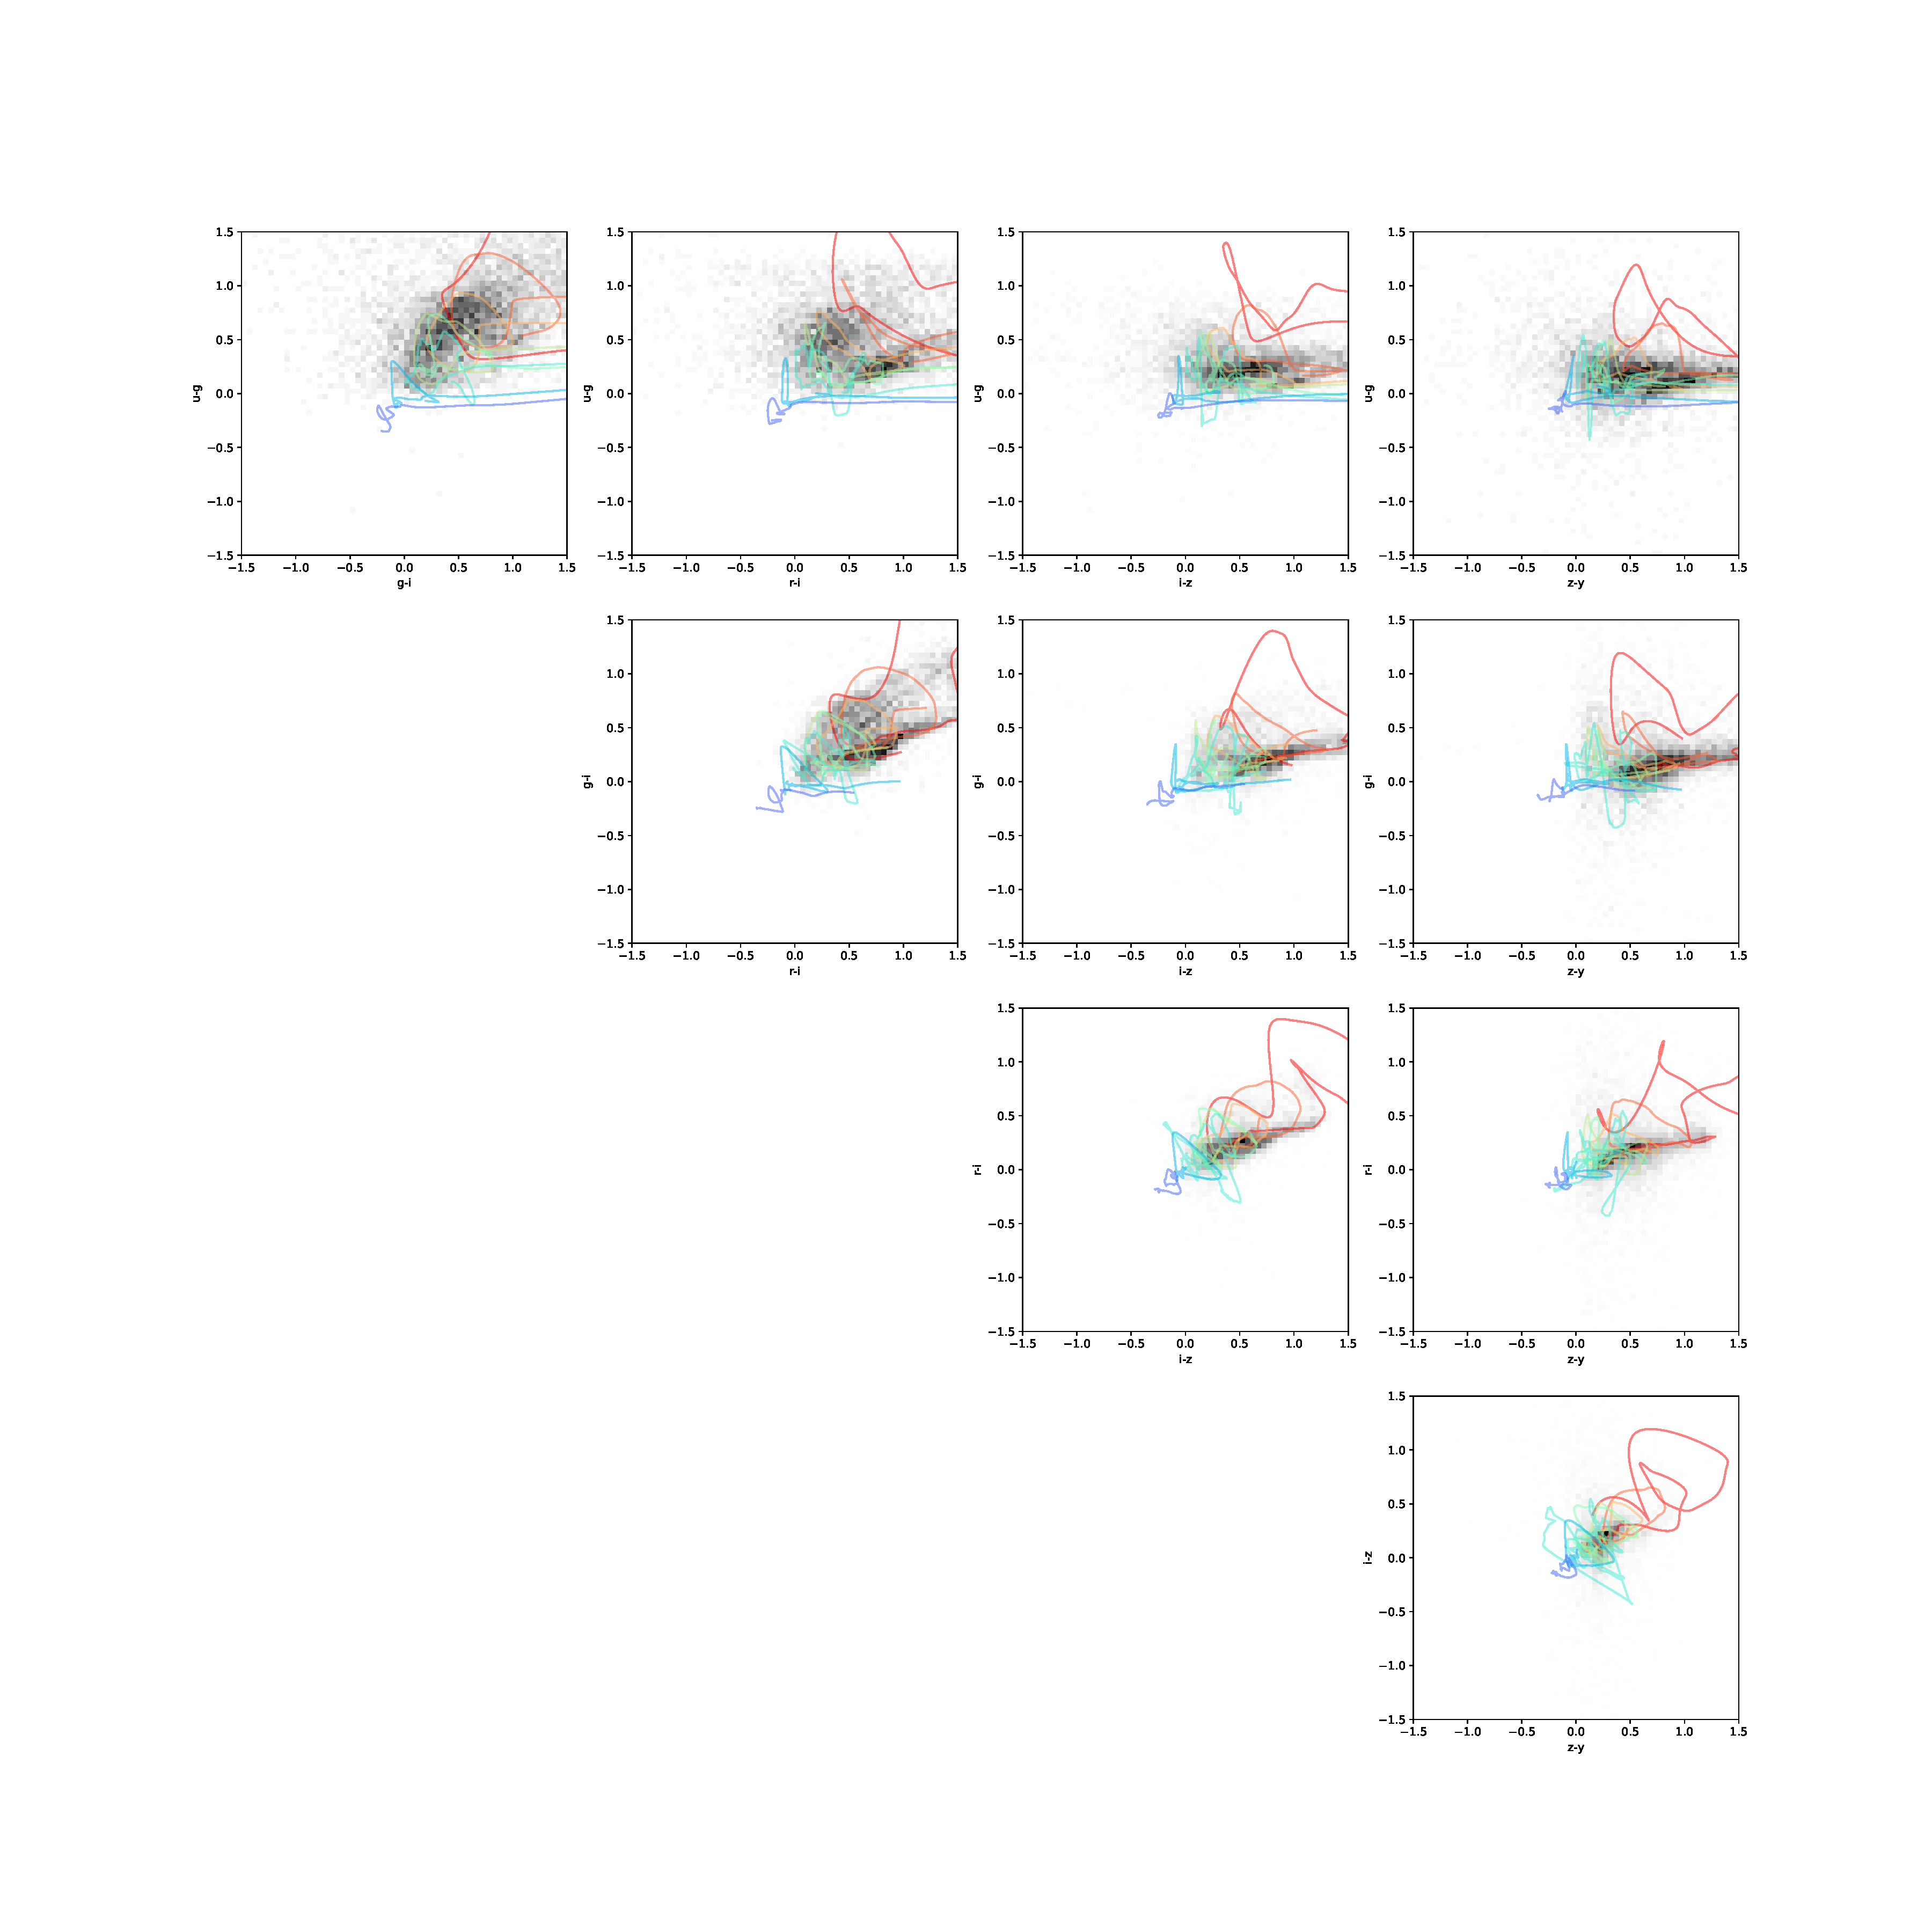
\includegraphics[width=\linewidth]{figures/color_v_color.pdf}
    \caption{Color-color correlations for all objects in the `\dataset{test\_v1} dataset.  Colored lines represent the expected colors for the eight ``CWWSB'' SEDs described in Sec.~\ref{sec:method:template}, and should very roughly show the predicted color evolution expected for our galaxy sample.}
    \label{fig:dp_color_v_color}
\end{figure*}

\pagebreak

\subsection{Redshift reference sample}
\label{sec:data:reference}

The \photoz estimation algorithms in RAIL require highly accurate and precise redshift estimates cross-matched to the DP1 photometric catalog to provide labeled \dataset{training} data sets.  We created such datasets using data drawn from publicly available catalogs in the ECDFS, comprising galaxies with known spectroscopic redshifts, grism redshifts, and high-quality \photoz's from deep multi-band imaging.  These training sets enable machine learning models within RAIL to learn the mapping between galaxy colors and redshifts, enabling \photoz estimation for every galaxy detected in DP1.

\begin{figure*}[b]
    \centering
    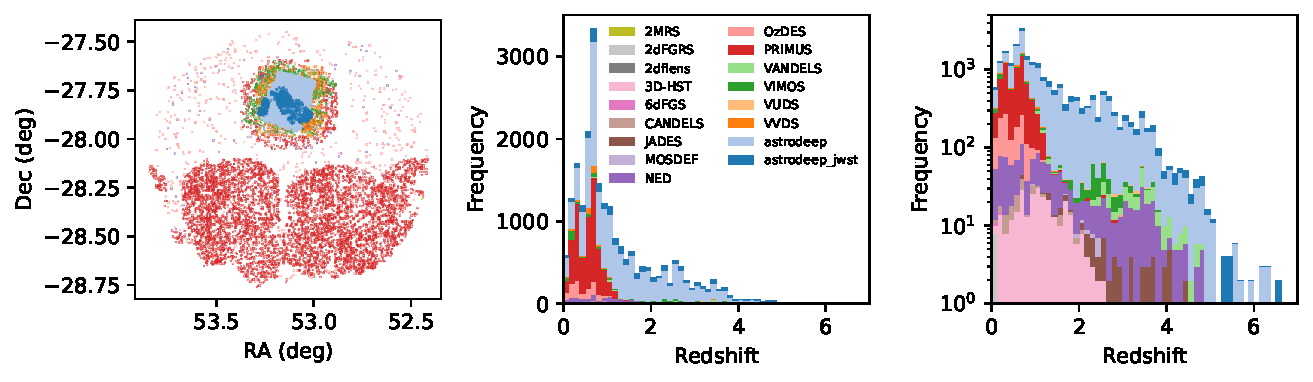
\includegraphics[width=\linewidth]{figures/redshift_reference_cat.pdf}
    \caption{
        Redshift reference sample in ECDFS.
        Left: Locations of DP1 galaxies cross-matched to objects in each reference catalog (using color scheme from middle panel).
        Many of the sets overlap in the densely-covered GOODS-S field.
        Middle: Redshift distribution of objects in the reference catalogs.
        Right: Same as middle panel with a log scale on the y-axis.
    }
    \label{fig:reference-sample}
\end{figure*}

The reference data set used to train \photoz estimation algorithms can have an outsize impact on the resulting \photoz estimates, particularly for machine learning based methods.  In many ways, the galaxies with known redshifts define the flux/color to distance relation by tracing out the mapping from empirical magnitudes to redshift that the algorithms ``learn''.  As such, the details of the construction of the reference sample is very important.  In an ideal case, we would prefer to have a ``representative'' sample of redshifts, i.~e.~a fair sampling in terms of the color and magnitude distribution for all galaxies; however, due to the practicalities of spectrographs and expensive telescope time investment needed for deep spectroscopic campaigns, we must deal with incomplete training samples, particularly for faint and high redshift objects.  We must also determine which datasets contain ``secure'' redshifts that meet some confidence threshold, and whether to include datasets from grism and many-band \photoz estimates that may contain a small fraction of incorrect redshift identifications.  We continue to refine our reference sample definition, and we may include or exclude additional samples as we investigate system performance, this note represents a current best effort, but the final selection will likely evolve.  There are also some concerns of imprinted sample variance, as the deep six-band data of DP1 is concentrated in the single ECDFS field.  Future Rubin data will cover multiple widely separated deep fields containing rich spectroscopic datasets, which will mitigate these concerns, but they may be an issue for the current DP1 estimates.


\subsubsection{ECDFS redshift datasets}
\label{sec:data:prelim}

We have compiled and used two redshift samples in the ECDFS, (a preliminary version and a reference sample), consisting of spectroscopic-, grism-, and high-quality multiband photometric-redshifts (Fig.~\ref{fig:reference-sample}).   

This reference sample is used to train machine learning \photoz estimators and evaluate \photoz performance.
The component redshift catalogs (described below) were combined into a single reference catalog and their respective quality flags were homogenized by defining a redshift ``confidence'' (more on this below).

When combining the component redshift catalogs, sources within $0.75''$ were identified as duplicates.
For these sources only the highest quality redshift is kept, i.e. spectroscopic redshifts are preferred over grism redshifts, which are preferred over \photoz's, and higher confidence values are preferred for redshifts of the same type.
The redshift reference catalog was then cross-matched to the ComCam DP1 catalog using a radius of $0.75''$.

Confidence, which takes values between 0.0 and 1.0, is loosely defined as the fractional probability that an individual redshift estimate is correct.
Most of the spectroscopic sets provide these estimates for their redshifts.
For the few that don't we assigned the confidence 0.95.
For the grism and multiband \photoz surveys, we set the confidence equal to $1 - f_\text{out}$, where $f_\text{out}$ is the reported outlier rate of these catalogs.
To facilitate custom quality cuts, the catalog contains flags indicating whether each redshift originates from spectroscopy (\code{type == ''s''}), grism (\code{''g''}), or multiband \photoz (\code{''p''}), as well as confidence values.
Note redshifts from grism and \photoz surveys, however, have larger scatter and bias than spectroscopic surveys (and possible incorrect redshifts if the redshift is based off of a single emission line), but these metrics are not captured by the confidence parameter.
We encourage readers to investigate the details of each component survey that comprise our reference catalog and apply their own quality cuts as suit their needs.
For example, if studying high-redshift galaxies, you might choose to include the multiband \photoz's, which increase the number of redshifts at $z > 2$ by a factor of~3 (Fig.~\ref{fig:redshift-by-type}).

We applied conservative cuts for our fiducial analyses, specifically \code{type == ''s''}, \code{confidence >= 0.95}, SNR $>= 10$ in the $i$ band (using \code{gaap1p0} fluxes).
We then did a random 80\%/20\% train/test split on this catalog, resulting in a training set of 4803 redshifts and a test set of 1201 redshifts.

\begin{table}[!p]
    \centering
    \begin{tabular}{lllll}
        \hline
        Survey & Type & Confidence & Matches& Reference \\
        \hline
        \hline
        2dFGRS & s & 1.00 & 3 & \citet{colless2001} \\
               &   & 0.99 & 4 & \\
               &   & 0.90 & 1 & \\
        2dflens & s & 1.00 & 1 & \citet{blake2016} \\
        2MRS & s & 0.95 & 1 & \citet{huchra2012} \\
        6dFGRS & s & 0.98 & 2 & \citet{jones2009} \\
        3D-HST & g & 0.99 & 5 & \citet{momcheva2016} \\
               &   & 0.95 & 277 & \\
        ASTRODEEP & s & 1.00 & 4165 & \citet{merlin2021} \\
                  & p & 0.97 & 8212 & \\
        ASTRODEEP-JWST & s & 1.00 & 594 & \citet{merlin2024} \\
                       & p & 0.92 & 628 & \\
                       &   & 0.90 & 455 & \\
        CANDELS & s & 1.00 & 53 & \citet{kodra2023} \\
                & p & 0.93 & 6 & \\
        JADES & s & 0.99 & 11 & \citet{deugenio2025} \\
              &   & 0.95 & 34 & \\
              &   & 0.90 & 24 & \\
        MOSDEF & s & 0.99 & 9 & \citet{kriek2015} \\
        NED & s & 0.95 & 847 & \citet{helou1991} \\
        OzDES & s & 0.99 & 897 & \citet{lidman2020} \\
        PRIMUS & g & 0.92 & 3653 & \citet{cool2013} \\
               &   & 0.85 & 1687 & \\
        VANDELS & s & 1.00 & 196 & \citet{garilli2021} \\
        VIMOS & s & 1.00 & 499 & \citet{balestra2010} \\
                  &   & 0.95 & 43 & \\
        VUDS & s & 1.00 & 9 & \citet{tasca2017} \\
             &   & 0.95 & 9 & \\
             &   & 0.80 & 3 & \\
        VVDS & s & 1.00 & 101 & \citet{lefevre2013} \\
             &   & 0.95 & 193 & \\
        \hline
        Total & s & & 7699 & \\
              & g & & 5622 & \\
              & p & & 9301 & \\
              & all & & 22622 & \\
        \hline
    \end{tabular}
    \caption{
        Component surveys of the redshift reference sample.
        Redshift type is denoted\\ s = spectroscopic, g = grism, p = multiband \photoz.
        Note for our fiducial analyses we applied conservative cuts on this catalog.
        Specifically, \code{type == ''s''}, \code{confidence >= 0.95}, SNR $>= 10$ in the $i$ band (using \code{gaap1p0} fluxes).
    }
    \label{tab:reference-sample}
\end{table}

\begin{figure}
    \centering
    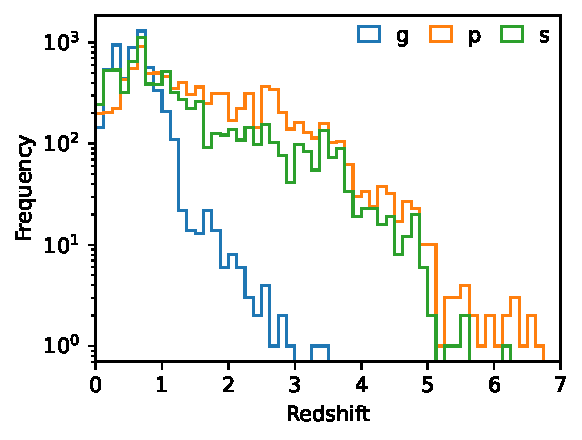
\includegraphics{figures/redshift_distribution_by_type.pdf}
    \caption{
        Redshift distribution of the reference catalog by redshift type, denoted s = spectroscopic, g = grism, p = multiband \photoz.
    }
    \label{fig:redshift-by-type}
\end{figure}

The \selection{match\_prelim} selection used in the \dataset{train\_v1} and \dataset{test\_v1} 
includes all spectroscopic and grism galaxies in the ``match\_ecfds'' catalog, without applying 
any confidence cut, and only required SNR $>= 5$ in the $i$ band (using \code{psf} fluxes).   
This selection also dropped all galaxies with NaN magnitude in any of the six bands.
We randomly selected 7,000 objects for the \dataset{train\_v1} and assigned the remaining 2,438 to the 
\dataset{test\_v1}  dataset. Although we used these datasets extensively in V1 of this technote, 
we intend to update the note to use the \dataset{train\_v2} and \dataset{test\_v2} as soon as possible, 
ideally in the first week of July, 2025.


\subsubsection{DESI Data Release 1 spectroscopic redshift dataset}
\label{sec:data:desi}

We also use data from the DESI Data Release \citep{desi-dr1} to act as an independent validation data set as it overlaps the \field{Rubin SV 38-7} (\field{SV\_38}) field.
The observations of this field are centered on the Abell 360 galaxy cluster which is located at $z=0.22$~\citep{A360z}.
We cross-matched the DESI Bright Galaxy Sample (BGS) \citep{BGS}, Emission Line Galaxy (ELG) \citep{ELG}, and Luminous Red Galaxy (LRG) \citep{LRG} samples against the DP1 catalog using a radius of 0.5'' producing 2728  matches with 398 from the BGS sample, 1421 from ELG, and 909 from LRG.
The area of overlap and the three subsamples are shown in Fig.~\ref{fig:desi-overlap}.
This spans a redshift range of 0 to 1.6 and \textit{i}-mag of 14 to 23.9 as shown in Fig.~\ref{fig:desi-subsample-hist}; the bump at $z\approx0.25$ can be attributed to the cluster at the center of the field.


\begin{figure}[ht]
    \centering
    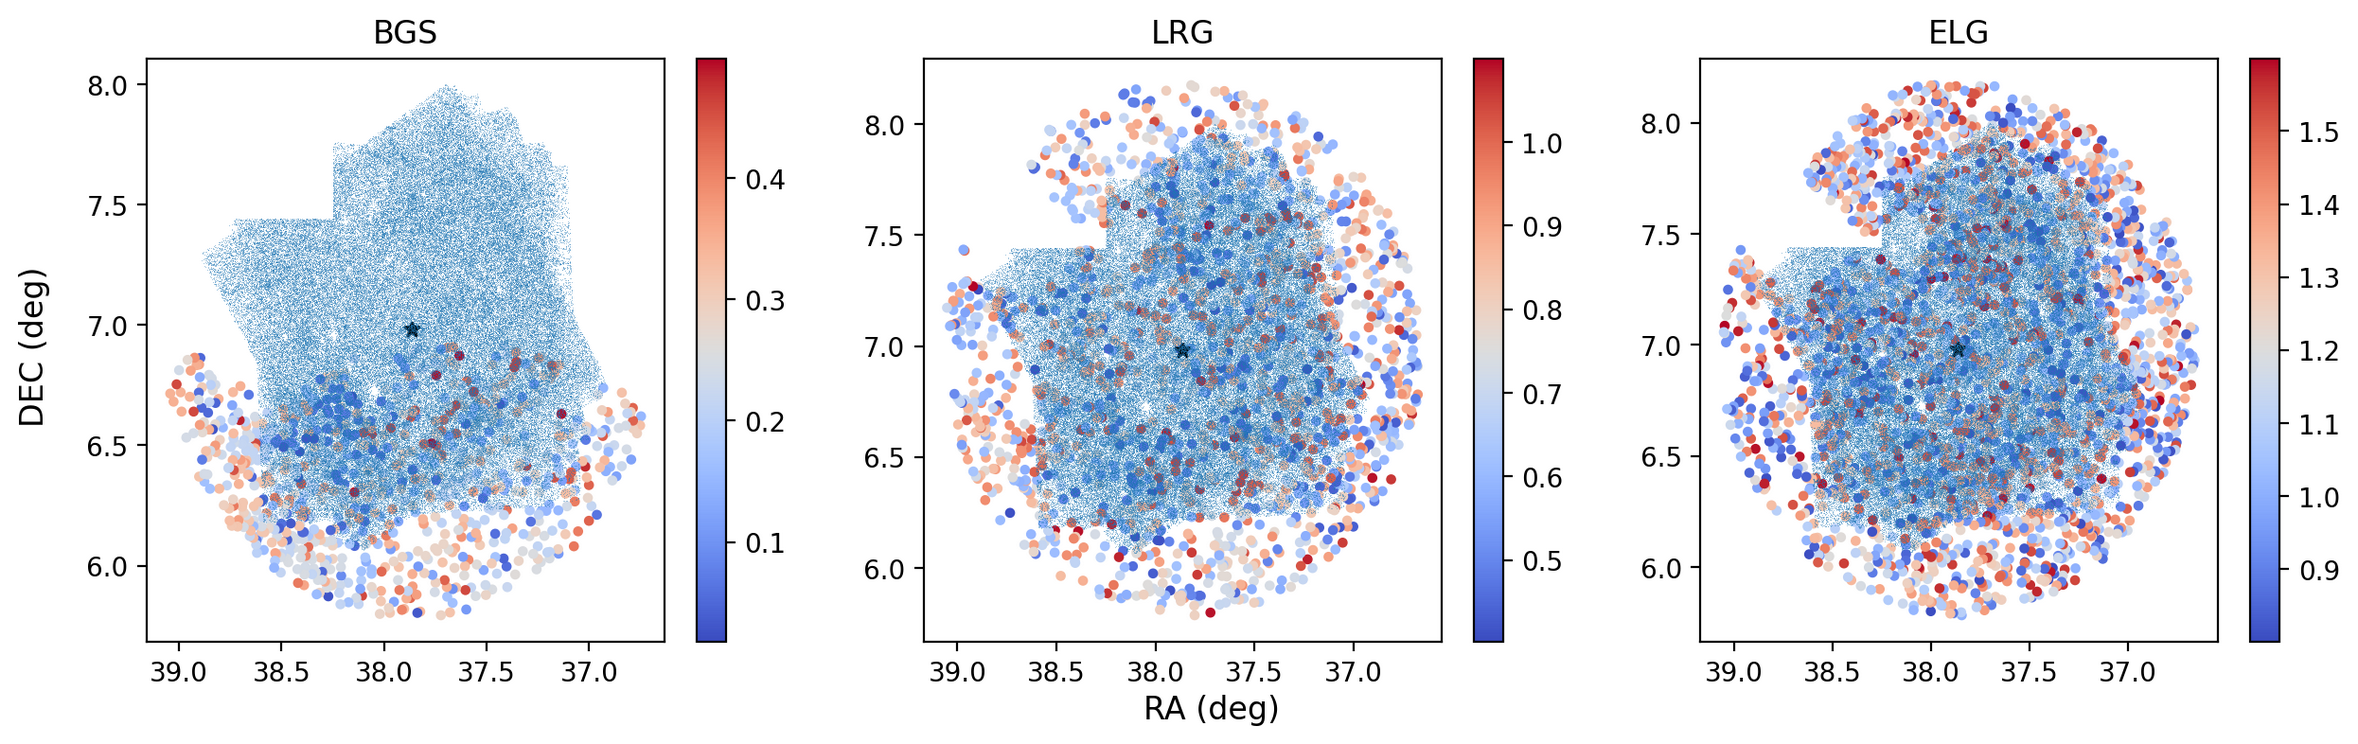
\includegraphics[width=\linewidth]{figures/desi_sample_overlap.png}
    \caption{Overlap between the \field{SV\_38} sample and DESI subsamples. In all plots, the small blue dots are DP1 objects from ComCam and we overlay, from left to right, the BGS, LRG, and ELG subsamples with points color-coded by redshift. Each sample probes a different redshift range and is shown with the color bar to the right of each panel.}
    \label{fig:desi-overlap}
\end{figure}

\begin{figure}]ht]
    \centering
    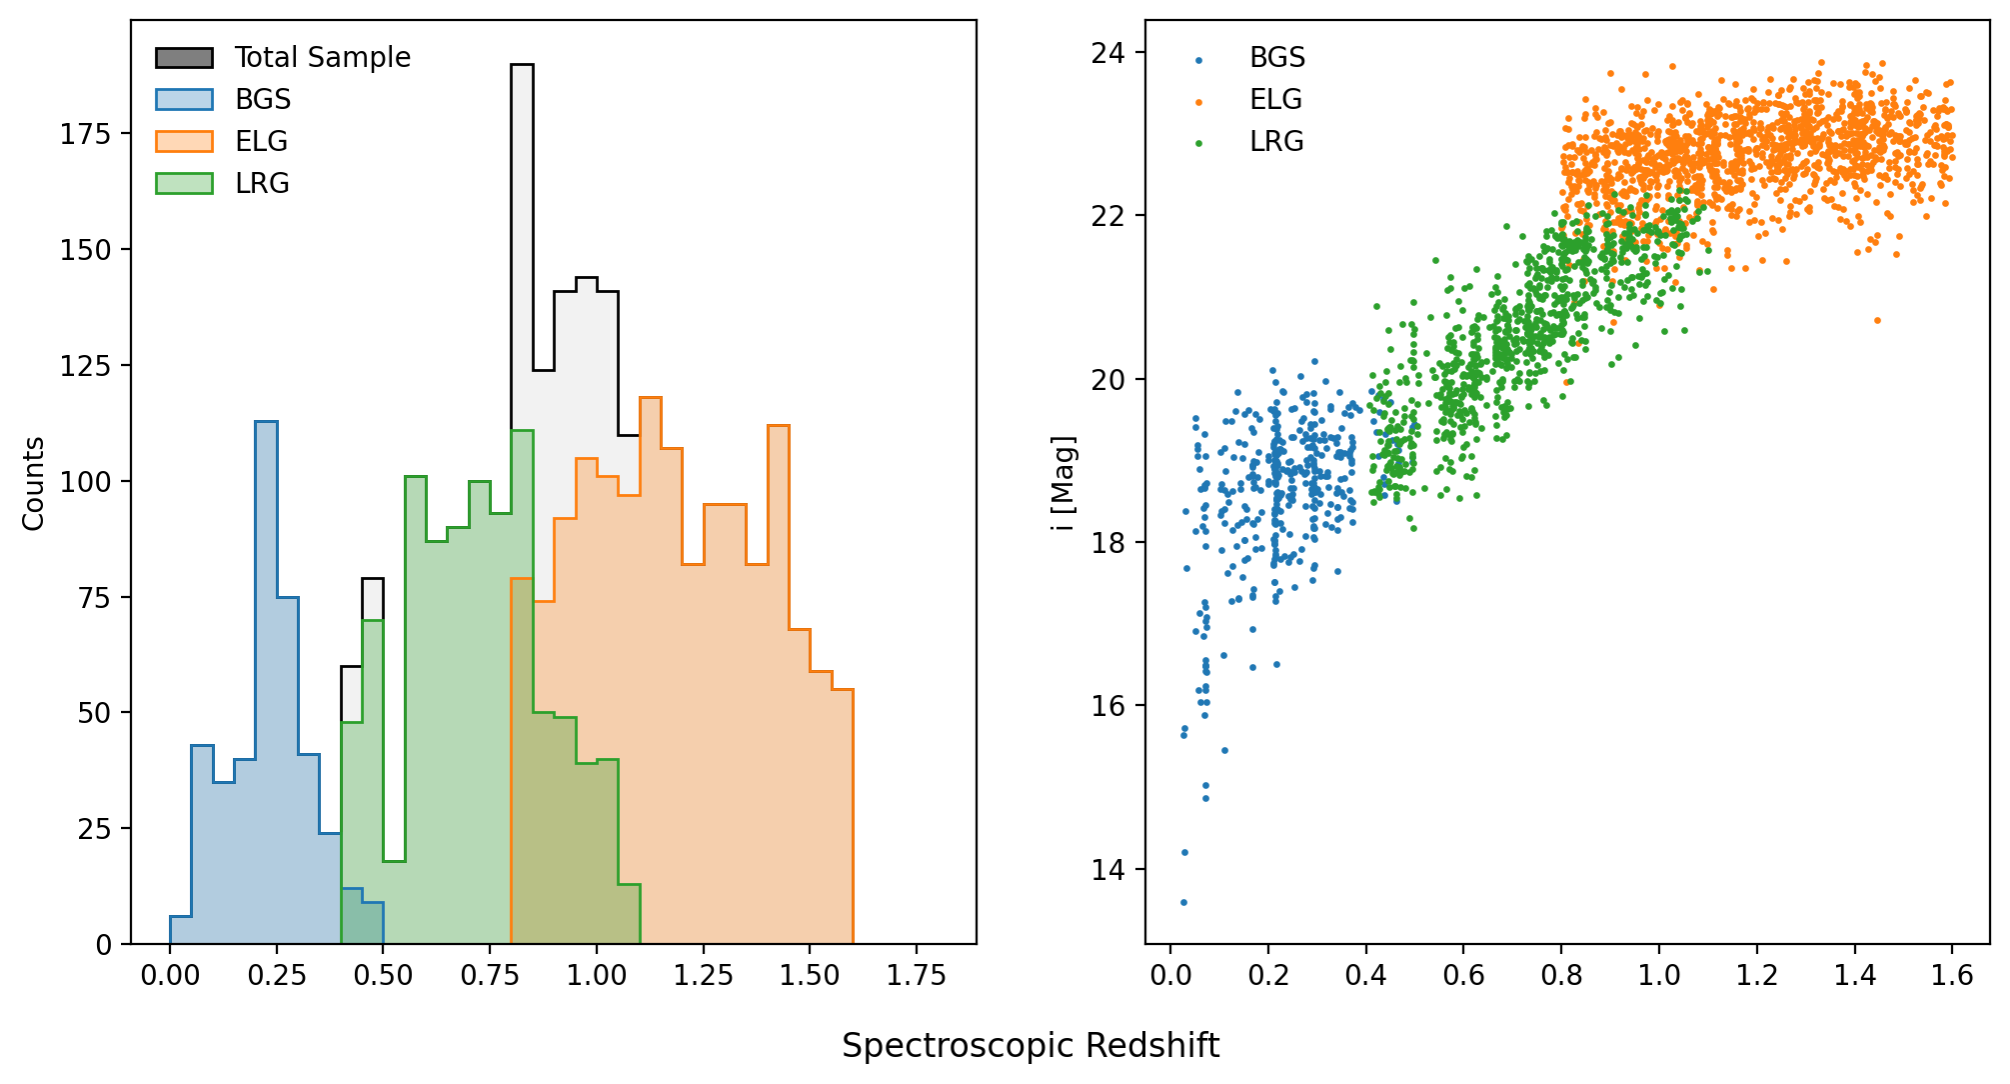
\includegraphics[width=.8\linewidth]{figures/desi_sample_histogram.png}
    \caption{Validation set on \field{SV\_38} from DESI BRG, ELG, and LRG samples. Left plot: the redshift distribution of the matched subsample with BGS in blue, ELG in orange, LRG in green, and the total matched distribution in black. Right plot: \textit{i}-band magnitude as measured by ComCam versus spectroscopic redshift for all DESI matches with subsamples shown using the same color scheme as left plot.}
    \label{fig:desi-subsample-hist}
\end{figure}

If an object was included in multiple samples, when matching we restrict to the one with the largest weight as calculated by DESI DR1.
The \field{SV\_38} field was observed in \textit{g} (44 visits), \textit{r} (55 visits), \textit{i} (57 visits) and \textit{z} (27 visits) bands restricting our validation to the 4 band models.
Furthermore, the incomplete overlap with the BGS sample limits our ability to validate on redshifts below $z=0.5$. 


\section{Methodology}
\label{sec:method:0}

We used the RAIL as the core tool for training and applying \photoz estimation models.   We also used RAIL to evaluate the model performance through a suite of diagnostic metrics using \photoz point estimates, including redshift bias, scatter (e.g., normalized median absolute deviation), and catastrophic outlier rate and to make diagnostic plots of the algorithm's performance.  Specifically, we used the methodology described below to evaluate all the algorithms listed in Tab.~\ref{tab:alg}.

As part of the Rubin \photoz roadmap process, \code{KNN} and \code{BPZ} were chosen as ``testing algorithms'' from the shortlist of algorithms considered in~\citep{DMTN:049}, the expectation is that these will supported by project data management team for Data Preview 2,  while the others will be supported by the wider community, the RAIL development team and DESC collaboration.


\begin{table*}[ht]
\centering
\begin{tabular}{lll}
 \hline
    Algorithm name  & Home package & Reference\\
 \hline
 \hline
 \multicolumn{3}{c}{Project Supported Testing} \\ 
  \code{BPZ} & \href{https://github.com/LSSTDESC/rail_bpz}{\code{rail-bpz}} & \citet{Benitez:2000}\\
 \code{KNN} & \href{https://github.com/LSSTDESC/rail_sklearn}{\code{rail-sklearn}} & RAIL Paper\\
 \multicolumn{3}{c}{Community Supported} \\   
 \code{CMNN} & \href{https://github.com/LSSTDESC/rail_cmnn}{\code{rail-cmnn}} & \citet{Graham:2018}\\
 \code{DNF} & \href{https://github.com/LSSTDESC/rail_dnf}{\code{rail-dnf}} & \citet{2016MNRAS.459.3078D}\\
 \code{FlexZBoost}  & \href{https://github.com/LSSTDESC/rail_flexzboost}{\code{rail-flexzboost}} & \citet{Izbicki:2017}\\
 \code{GPz} & \href{https://github.com/LSSTDESC/rail_gpz_v1}{\code{rail-gpz-v1}} & \citet{Almosallam:2016}\\
 \code{LePHARE} & \href{https://github.com/LSSTDESC/rail_lephare}{\code{rail-lephare}} & \citet{1999MNRAS.310..540A}\\
 \code{TPZ} & \href{https://github.com/LSSTDESC/rail_tpz}{\code{rail-tpz}} & \citet{Carrasco-Kind:2013}\\
 \hline
\end{tabular}
\caption{
Summary of the pre-wrapped estimators/summarizers/classifiers used in this paper and described detail in~\citep{RAIL}.}
\label{tab:alg}
\end{table*}

For each algorithm, we trained \photoz models using the reference datasets described in Sec.~\ref{sec:data:reference}.   Specifically, we used the \code{rail\_project} package (see \ref{sec:method:rail_project} to run RAIL’s \href{https://github.com/LSSTDESC/rail_pipelines/blob/main/src/rail/pipelines/estimation/pz_all.py}{PzPipeline}.  The pipeline consists of ``Informing'' or training the models on the ``training'' dataset, and using those models in ``Estimation'' and ``Evaluation'' stages on the reserved ``test'' dataset to evaluate the algorithm performance.  We also used \code{rail\_project} to run RAIL’s  \href{https://github.com/LSSTDESC/rail_pipelines/blob/main/src/rail/pipelines/estimation/estimate_all.py}{EstimatePipeline}, to perform the photometric redshift estimation on the unlabeled data sets for all of the algorithms.

In this work we are only using the magnitudes in the six (or four) available Rubin bands as inputs to the photometric estimation.  We do not use other inputs, such as object size or morphology, or photometry from other surveys.   As stated in
Sec.~\ref{sec:data:dp1:properties}, we systematically use the \texttt{gaap1p0} version of the fluxes, as these are considered the most reliable for color estimation.


\subsection{Template fitting based estimators}
\label{sec:method:template}

RAIL’s template-based fitting algorithms (\code{Lephare} and \code{BPZ}, see references in Tab.~\ref{tab:alg} for more details) estimate photometric redshifts by comparing observed galaxy photometry to a set of predefined theoretical or empirical galaxy templates.  These templates represent a range of galaxy spectral energy distributions (SEDs) that are meant to span the expected range of galaxy types observed in the Universe.  Synthetic model fluxes are computed by red-shifting each SED to a set grid of values and convolving with the Rubin filter curves,  which characterizes the expected variation in observed colors with redshift.  Our algorithms calculate the chi-square/likelihood for each SED at each grid point by comparing the model fluxes in our photometric bands to the observed fluxes and uncertainties.  This process enables the algorithm to determine the relative likelihood for each redshift for a given galaxy by identifying the template that best matches its observed color signature.  An optional empirical Bayesian prior can also be applied to produce a posterior probability rather than a straight likelihood if information on the expected distributions are available.  The training phase for these algorithms consist mostly of preparing pre-computed tables for the expected fluxes in each filter band for each SED template. 

Two sets of templates are included in the \code{rail\_base} software package and used in this note: the ``CWWSB'' templates that are the default templates used by \code{rail\_bpz} and described in \citet[]{Coe:06}, consisting of eight total SEDs, one Elliptical template, two Spiral templates, and five Irregular/Starburst template.  In this note, these SEDs are used to compute synthetic colors that we compare to the observational data in Figures~\ref{fig:dp_color_v_redshift} and~\ref{fig:dp_color_v_color}, but are otherwise not used.  The second template set consists of those described in \citet[]{Ilbert:09}, consisting of 31 synthetic SEDs (including some that are ``interpolated'' between adjacent templates by taking the mean of the two SEDs).  These SEDs are included with \code{rail\_lephare} as ``COSMOS\_mod.list'' in the \code{lephare-data} package.  These SEDs are used by both template codes \code{rail\_bpz} and \code{rail\_lephare}.  The 31 base SEDs contain no internal dust extinction, \code{rail\_lephare} is configured to include dust automatically, while \code{rail\_bpz} required dust to be added explicitly, and additional SED templates that include internal extinction added to the input SED list. \code{LePhare} also includes a set of stellar and AGN SEDs, which are available in the \code{lephare-data} package.


\subsection{Machine learning based estimators}
\label{sec:method:machine_learning}

RAIL’s machine learning algorithms (\code{CMNN}, \code{DNF}, \code{FlexZBoost}, \code{GPZ}, \code{KNN}, \code{TPZ}) are described in detail in the publications listed in Tab.~\ref{tab:alg}.  In short these algorithms attempt to perform a regression analysis to estimate the redshift from the input photometric data.   It is a well-known limitation of machine learning algorithms that they exhibit biases when presented with non-representative data, or are asked to extrapolate results outside region of their training data.


\subsection{Analysis framework and bookkeeping software}
\label{sec:method:rail_project}

The \code{rail\_projects} software package within the RAIL ecosystem provides an essential framework for managing and organizing large-scale photometric redshift estimation workflows.  It acts as a project management and book-keeping tool that helps users streamline their research, especially when working with complex or large datasets, like those associated with the Rubin DP1 data.  The primary focus of \code{rail\_projects} is to offer a systematic way to track different stages of data processing, model training, evaluation, and results across multiple experiments, ensuring that all tasks are well-documented and reproducible.

Additionally, \code{rail\_projects} facilitates the management of large datasets by organizing data into structured directories and providing interfaces for batch processing.  It allows users to scale up their work to handle not only large catalogs of objects but also multiple datasets and redshift estimation tasks.  The package ensures that datasets and models are kept in sync across various stages, from raw input data to intermediate results to final outputs, and makes it easier to systematically export data coherent products.

\subsection{Data exploration and algorithm optimization}
\label{sec:method:optimization}

We explored dozens of different configuration settings, covering analysis choices such as which flux measurements to use, the machine learning hyper-parameters, which sets of SED templates to use, among others.   The \href{https://github.com/LSSTDESC/rail_project_config/blob/main/dp1/dp1.yaml}{dp1/dp1.yaml} configuration file (see Sec.~\ref{sec:products:configuration}) captures the set of configurations that we tested and labels each set into an analysis ``flavor'' to facilitate bookkeeping. 

After examining the performance of the algorithms under different configurations, we settled on a set of optimized parameters for each algorithm and on the \code{gaap\_1p0} fluxes to produce the best-effort catalogs for DP1.   These optimized configurations parameters are captured in the \href{https://github.com/LSSTDESC/rail_project_config/blob/main/dp1/dp1.yaml}{dp1/dp1\_v1.yaml} configuration file.


\subsection{Production of redshift catalogs}
\label{sec:method:redshift_catalogs}

We produced \photoz catalogs in two different software frameworks, both to test the software pipelines as well as to facilitate using associated tools to distribute the resulting data products. 


\subsubsection{Catalogs in the \code{rail\_projects} framework}
\label{sec:method:redshift_catalogs:rail}

We used \code{rail\_project} to run RAIL’s  \href{https://github.com/LSSTDESC/rail_pipelines/blob/main/src/rail/pipelines/estimation/estimate_all.py}{EstimatePipeline}, to perform the photometric redshift estimation on the unlabeled data sets for all of the algorithms.

Specifically, we used \code{rail\_project} to run all of the configuration flavors defined in the \href{https://github.com/LSSTDESC/rail_project_config/blob/main/dp1/dp1.yaml}{dp1/dp1.yaml} and \href{https://github.com/LSSTDESC/rail_project_config/blob/main/dp1/dp1.yaml}{dp1/dp1\_v1.yaml} configuration files.
The resulting data products are internally available as files at the USDF and NERSC as described in App.~\ref{sec:distribution:files}.   It is expected some of the products will be distributed via other methods in the near future (see App.~\ref{sec:distribution:linea} and App.~\ref{sec:distribution:lsdb}).


\subsubsection{Catalogs in the Rubin data management framework}
\label{sec:method:redshift_catalogs:dm}

We also used the \href{https://github.com/lsst-dm/meas_pz}{\code{meas\_pz}} and \href{https://github.com/lsst-dm/meas_pz}{\code{meas\_pz\_extensions}} software packages
to create \photoz catalogs in the Rubin data management framework.

Specifically, we imported trained models produced in the \code{rail\_project} into the DP1 data Butler and produced \photoz estimates for every object in DP1 for each algorithm.

We did this for the \texttt{baseline} analysis flavor, (consisting of ``out-of-the-box'' algorithms, with all settings at default values) and the optimized 6 band (\texttt{dp1\_optimze}) flavor defined in \href{https://github.com/LSSTDESC/rail_project_config/blob/main/dp1/dp1.yaml}{dp1/dp1\_v1.yaml}.
The resulting data products are internally available via data Butlers at USDF and NERSC as described in App.~\ref{sec:distribution:butler}.   As with the \code{rail\_projects} created catalogs, it is expected some of the products will be distributed via other methods in the near future (see App.~\ref{sec:distribution:linea} and App.~\ref{sec:distribution:lsdb}).


\section{Performance}
\label{sec:performance:0}

We evaluated all the algorithms listed in Tab.~\ref{tab:alg} for both scientific and technical performance.

\subsection{Redshift estimator performance}
\label{sec:performance:pz}

We primarily evaluated the performance using the ``test\_v1'' catalog which consist of 2,437 galaxies randomly drawn from the cross-match between the DP1 object catalog in ECDFS with the reference redshifts described in Sec.~\ref{sec:data:reference}.  Additionally, we cross matched the DP1 object catalog in the \field{SV\_38} field with the DESI DR1 BGS, LRG and ELG galaxies as a secondary validation set (``test\_DESI''). 

Specifically, we ran the \href{https://github.com/LSSTDESC/rail_pipelines/blob/main/src/rail/pipelines/estimation/pz_all.py}{PzPipeline}
(Inform $\rightarrow$ Estimate $\rightarrow$ Evaluate) to train models for per-object $p(z)$ estimation on the training data set, use those models to obtain \photoz estimates for the test data set, and then evaluate the performance of the photometric point-estimate of the redshift against the spectroscopic estimates.

For each algorithm, we produce a set of performance monitoring plots, described in Sec.~\ref{sec:products:peformance_plots}. In Fig~\ref{fig:perf_gold}, we show examples of these performance monitoring plots for two algorithms: \code{knn} and \code{bpz} for the 6-band models and using the mode for the specific point estimate. Fig.~\ref{fig:perf_gold_4_band} shows the performance monitoring of \code{knn} and \code{bpz} when 4-bands are used. In the scattering plot, the mean, standard deviation, 3$\sigma$ outliers and absolute outliers of 
\begin{equation}
\label{eq:dz}
    \Delta z = \frac{z_{\rm phot} - z_{\rm spec}}{1+z_{\rm spec}}
\end{equation}
are shown in legend. We summarized these statistics in Table~\ref{tab:photoz_metrics}.

\begin{figure*}
    \centering
    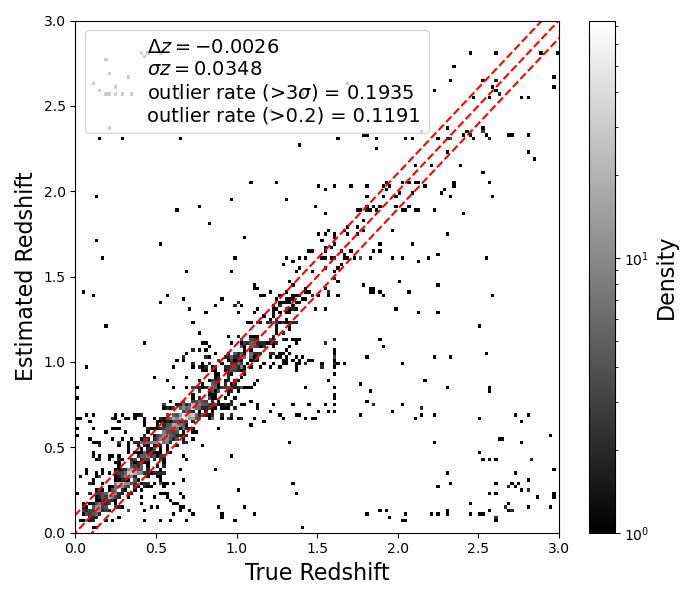
\includegraphics[width=0.45\linewidth]{figures/zestimate_v_ztrue_hist2d_knn.png}
    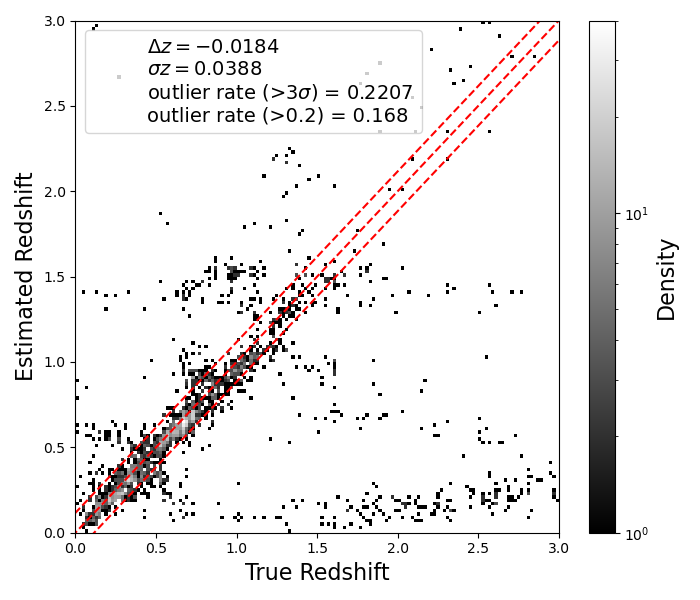
\includegraphics[width=0.45\linewidth]{figures/zestimate_v_ztrue_hist2d_bpz.png} \\
    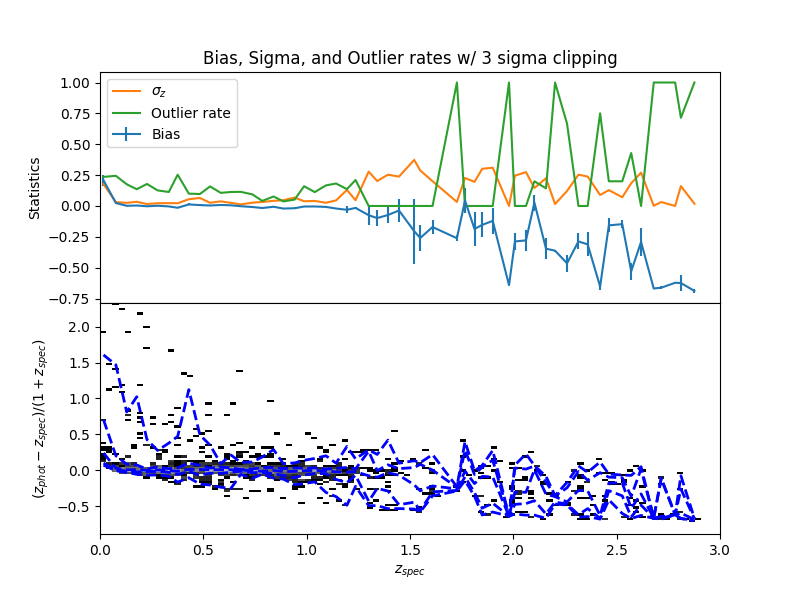
\includegraphics[width=0.45\linewidth]{figures/biweight_stats_v_redshift_knn.png}
    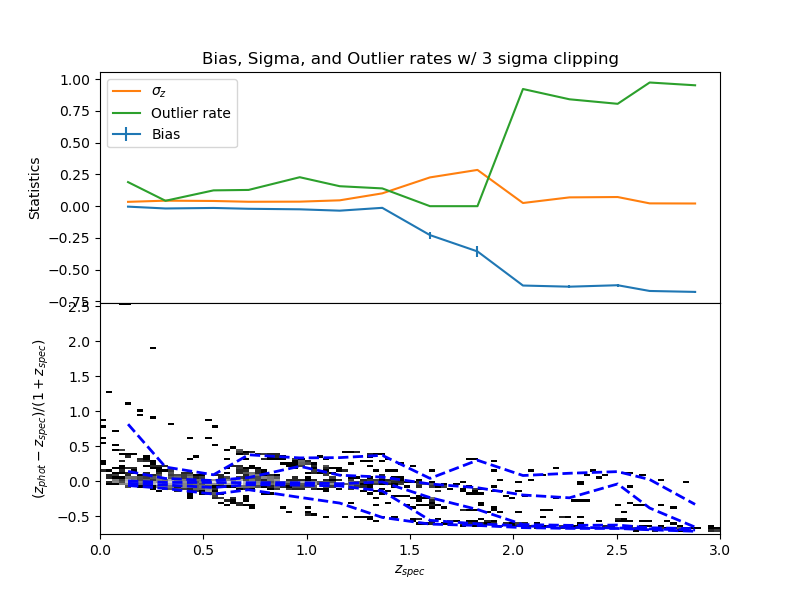
\includegraphics[width=0.45\linewidth]{figures/biweight_stats_v_redshift_bpz.png} \\
    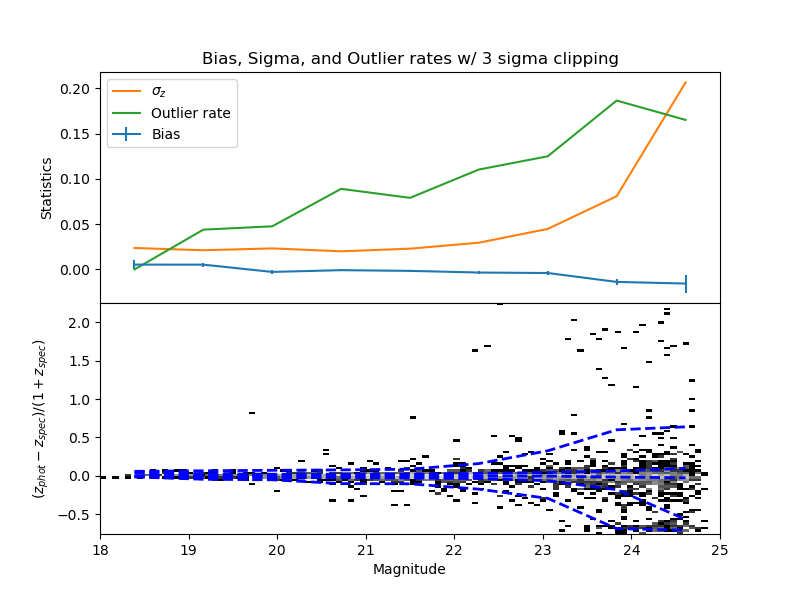
\includegraphics[width=0.45\linewidth]{figures/biweight_stats_v_mag_knn.png}
    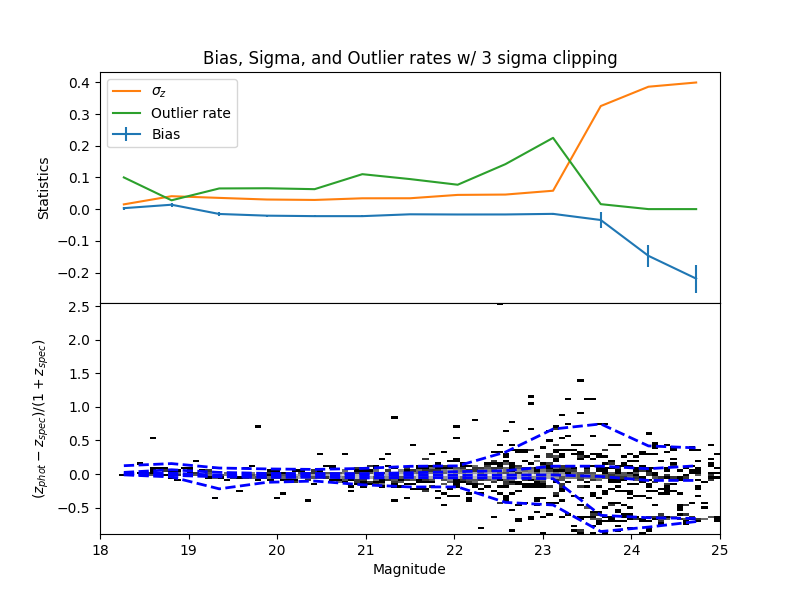
\includegraphics[width=0.45\linewidth]{figures/biweight_stats_v_mag_bpz.png}    
    \caption{Estimator performance on the ``gold'' (six-band') dataset.  Top row: photometric point estimate of the redshift versus spectroscopic redshift for \code{KNN} (left) and \code{bpz} (right).   Middle row: performance metrics, (width and bias of residual, and outlier rate) versus spectroscopic redshift.    Bottom row, performance metrics versus i-band magnitude.}
    \label{fig:perf_gold}
\end{figure*}

\begin{figure*}
    \centering
    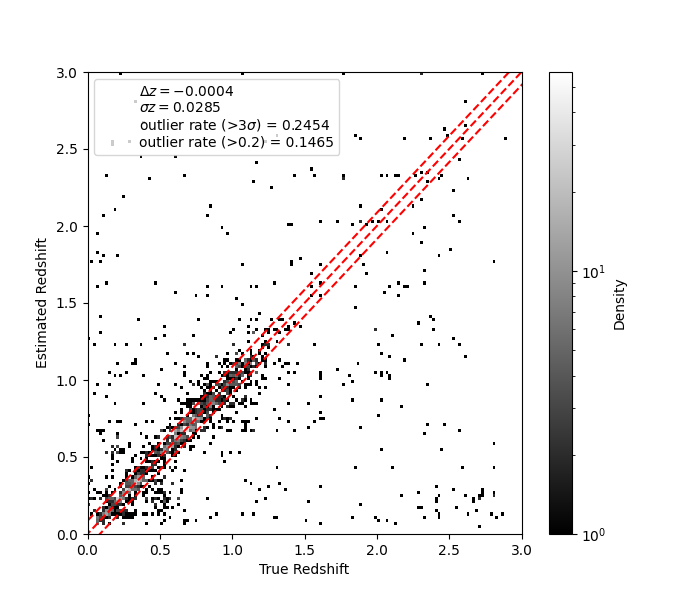
\includegraphics[width=0.45\linewidth]{figures/zestimate_v_ztrue_hist2d_knn_4.png}
    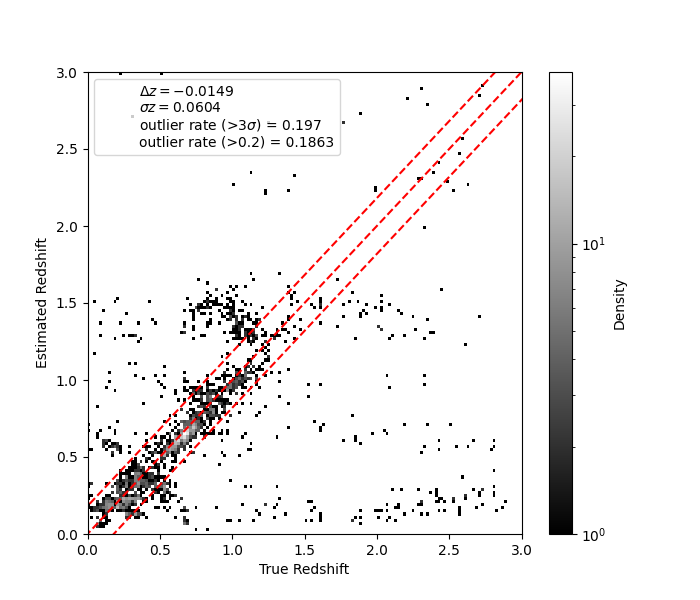
\includegraphics[width=0.45\linewidth]{figures/zestimate_v_ztrue_hist2d_bpz_4.png} \\
    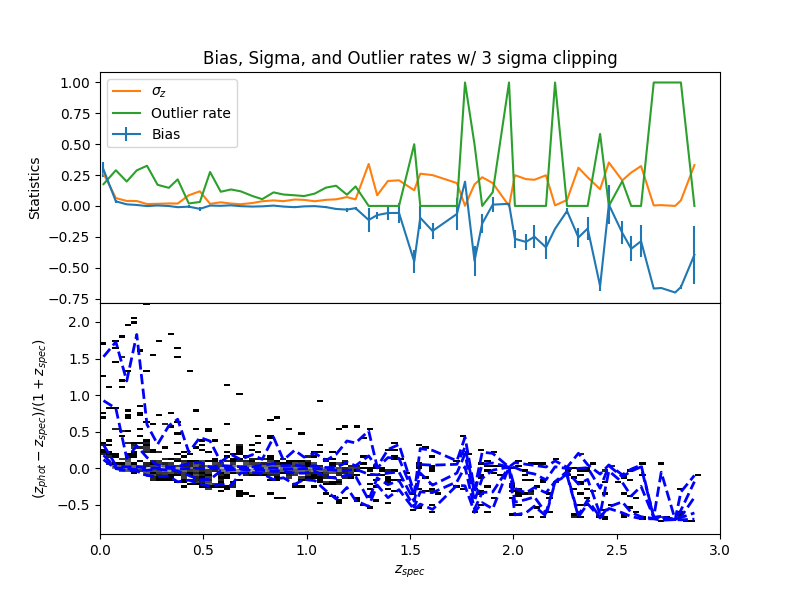
\includegraphics[width=0.45\linewidth]{figures/biweight_stats_v_redshift_knn_4.png}
    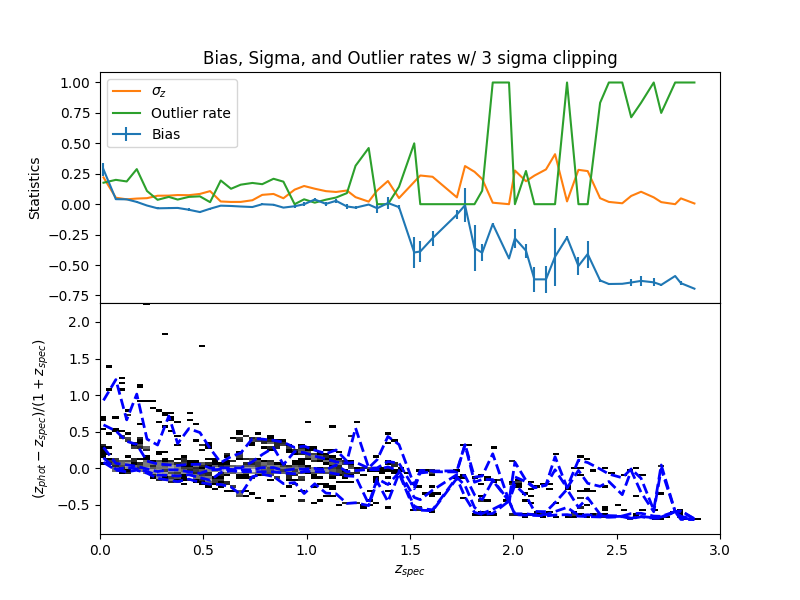
\includegraphics[width=0.45\linewidth]{figures/biweight_stats_v_redshift_bpz_4.png} \\
    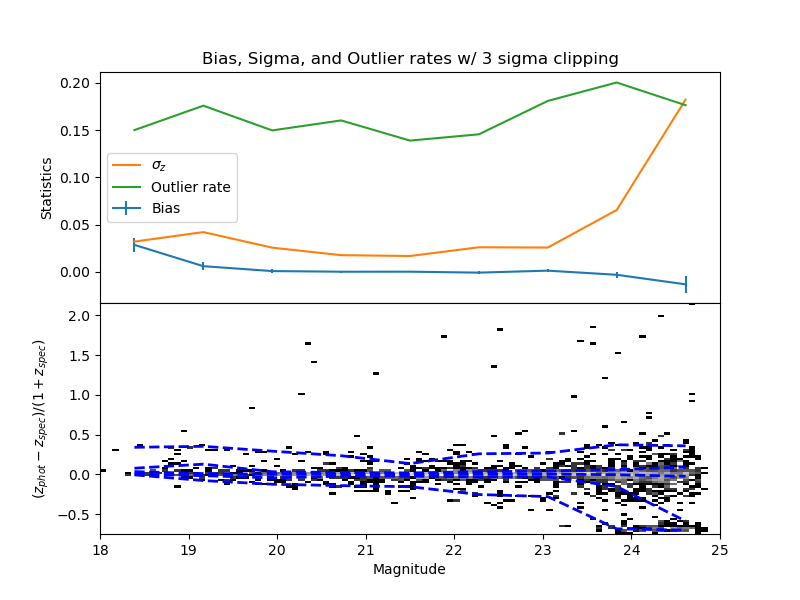
\includegraphics[width=0.45\linewidth]{figures/biweight_stats_v_mag_knn_4.png}
    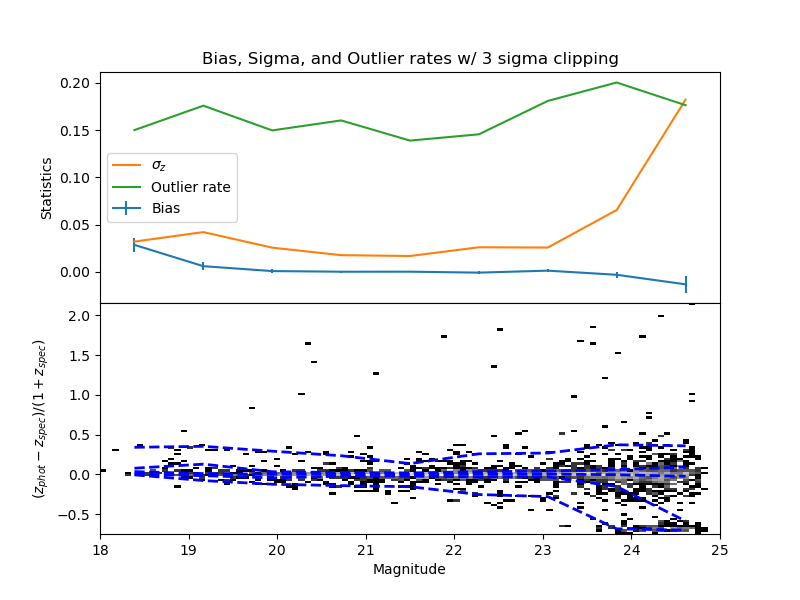
\includegraphics[width=0.45\linewidth]{figures/biweight_stats_v_mag_knn_4.png}    
    \caption{Estimator performance on the ``gold\_4\_band'' (four-band') dataset.  Top row: photometric point estimate of the redshift versus spectroscopic redshift for \code{KNN} (left) and \code{bpz} (right).   Middle row: performance metrics, (width and bias of residual, and outlier rate) versus spectroscopic redshift.    Bottom row, performance metrics versus i-band magnitude.}
    \label{fig:perf_gold_4_band}
\end{figure*}

\begin{table}[ht]
\centering
\caption{Performance metrics for \photoz algorithms using 6-band data, with 4-band results shown in parentheses.}
\begin{tabular}{lcccc}
\hline
\textbf{Algorithm} & \textbf{Bias} & \textbf{$\sigma$} & \textbf{3$\sigma$ Outlier Rate} & \textbf{$\Delta z>0.2$ Outlier Rate} \\
\hline
FlexZBoost & 0.000 (0.000) & 0.0246 (0.0274) & 0.215 (0.221) & 0.113 (0.124) \\
kNN        & -0.002 (-0.000) & 0.0301 (0.0285) & 0.205 (0.245) & 0.128(0.147) \\
CMNN       & 0.000 (-0.002) & 0.0369 (0.0729) & 0.227 (0.212) & 0.160 (0.226) \\
DNF        & -0.002 (-0.001) & 0.041 (0.0327) & 0.189 (0.215) & 0.138 (0.121) \\
TPZ        & -0.001 (-0.002) & 0.050 (0.0524) & 0.154 (0.156) & 0.117 (0.127) \\
GPz        & 0.032 (0.018) & 0.166 (0.106) & 0.056 (0.110) & 0.260 (0.198) \\
BPZ        & -0.018 (-0.015) & 0.0425 (0.060) & 0.198 (0.197) & 0.146 (0.186) \\
LePhare    & -0.012 (-0.015) & 0.0344 (0.0699) & 0.207 (0.175) & 0.139 (0.185) \\
\hline
\end{tabular}
\label{tab:photoz_metrics}
\end{table}



\subsubsection{Redshift estimation quality flags}
\label{sec:performance:pz:flag}

Applying a simple cut on the RMS of the $p(z)$ distribution can dramatically reduce the catastrophic outlier rate.  In Fig.~\ref{fig:perf_quality_cut} we show how the efficiency and purity obtained on the test sample varies with a single additional cut, $x$ in $\sigma_{p(z)} < x$.   In Fig.~\ref{fig:scatter_quality_cut} we show how applying a cut at $\sigma_{p(z)} < 0.15$ improves the scatter of the photometric redshift point-estimate versus spectroscopic redshift distribution.  As fainter objects and objects at higher redshift often have larger $p(z)$ RMS values, cuts on RMS will likely result in relative shifts in the magnitude and redshift distribution depending on the cut value.

\begin{figure*}
    \centering
    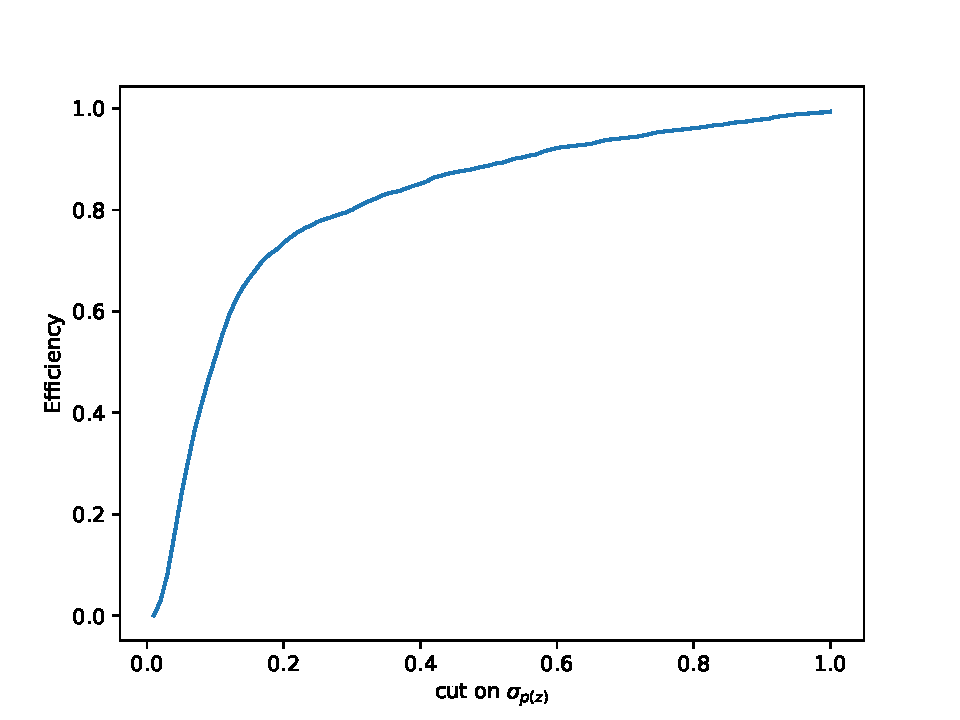
\includegraphics[width=0.45\linewidth]{figures/efficiency.pdf}
    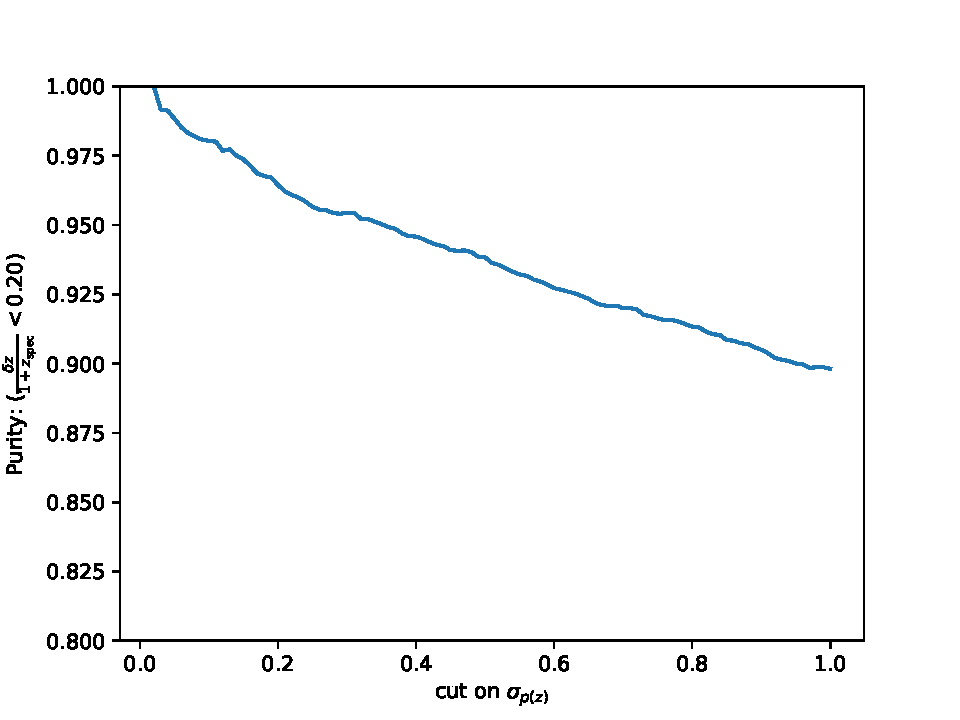
\includegraphics[width=0.45\linewidth]{figures/purity.pdf} \\
    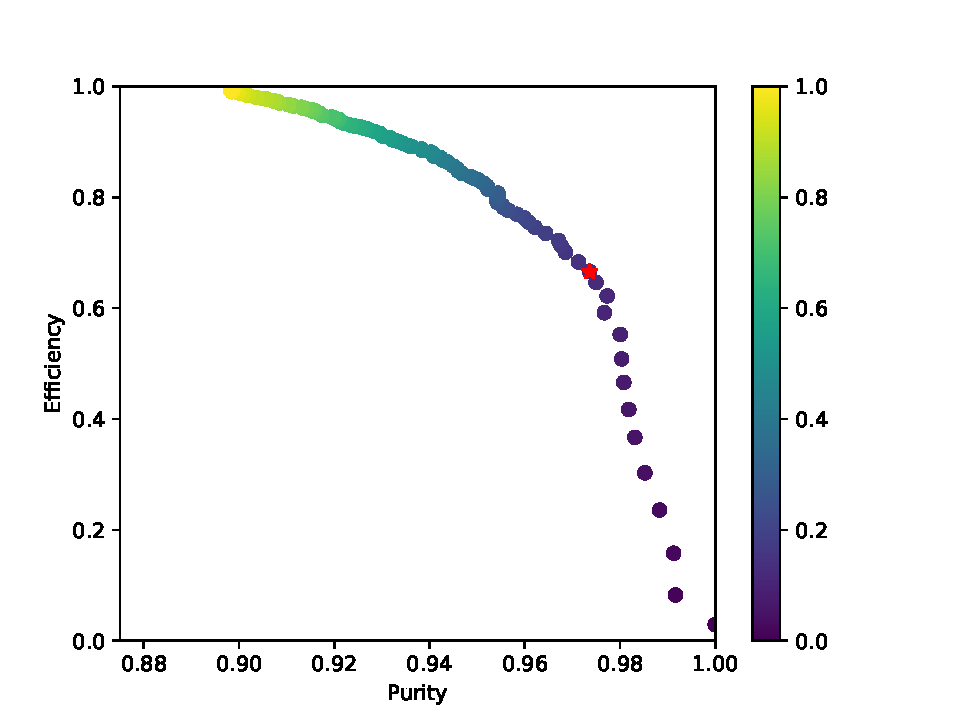
\includegraphics[width=0.45\linewidth]{figures/purity_v_effic.pdf} \\
    \caption{Efficiency (top left) and ``purity'', i.e., fraction of objects with $\frac{\delta z}{1 + z_{\rm spec}} < 0.20$) (top right) versus quality cut, $x$ in $\sigma_{p(z)} < x$.   Bottom, purity version efficiency with cut value shown by the color scale.   The red star shows the point for a cut value  $\sigma_{p(z)} < 0.15$.}
    \label{fig:perf_quality_cut}
\end{figure*}

\begin{figure*}
    \centering
    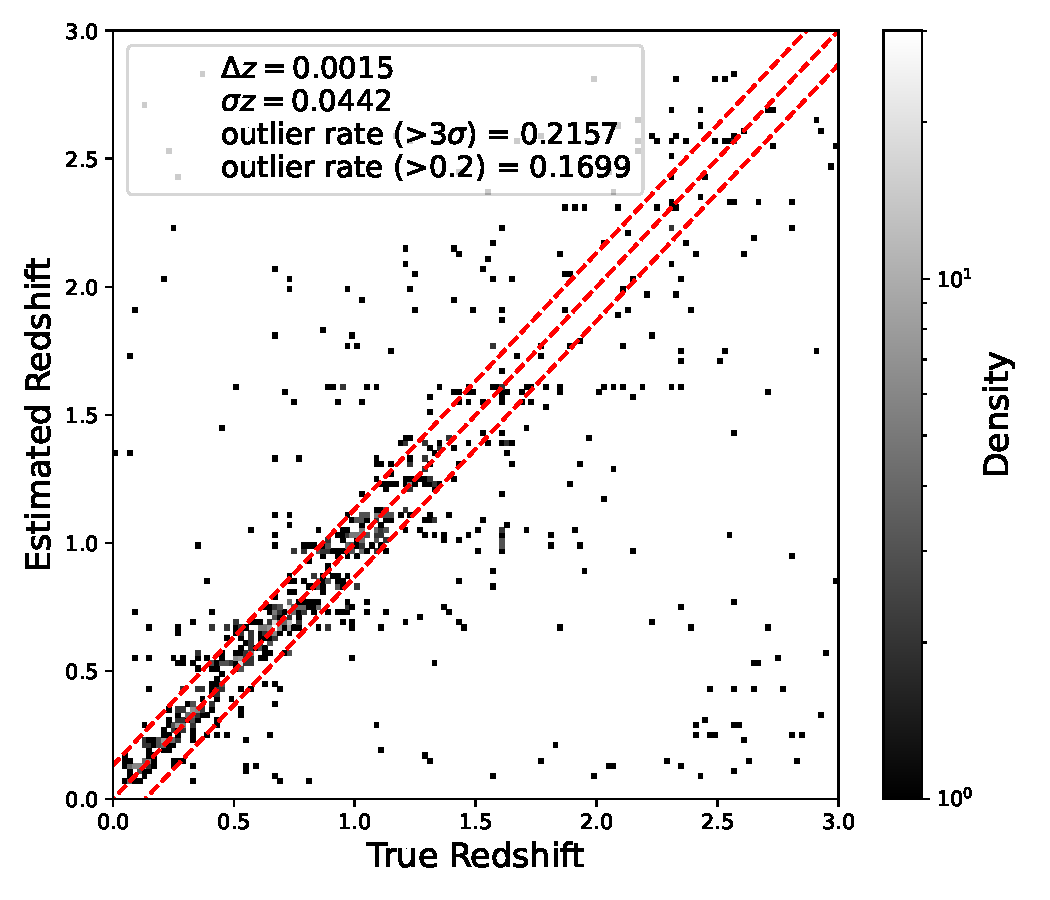
\includegraphics[width=0.45\linewidth]{figures/tpz_scatter_orig.pdf}
    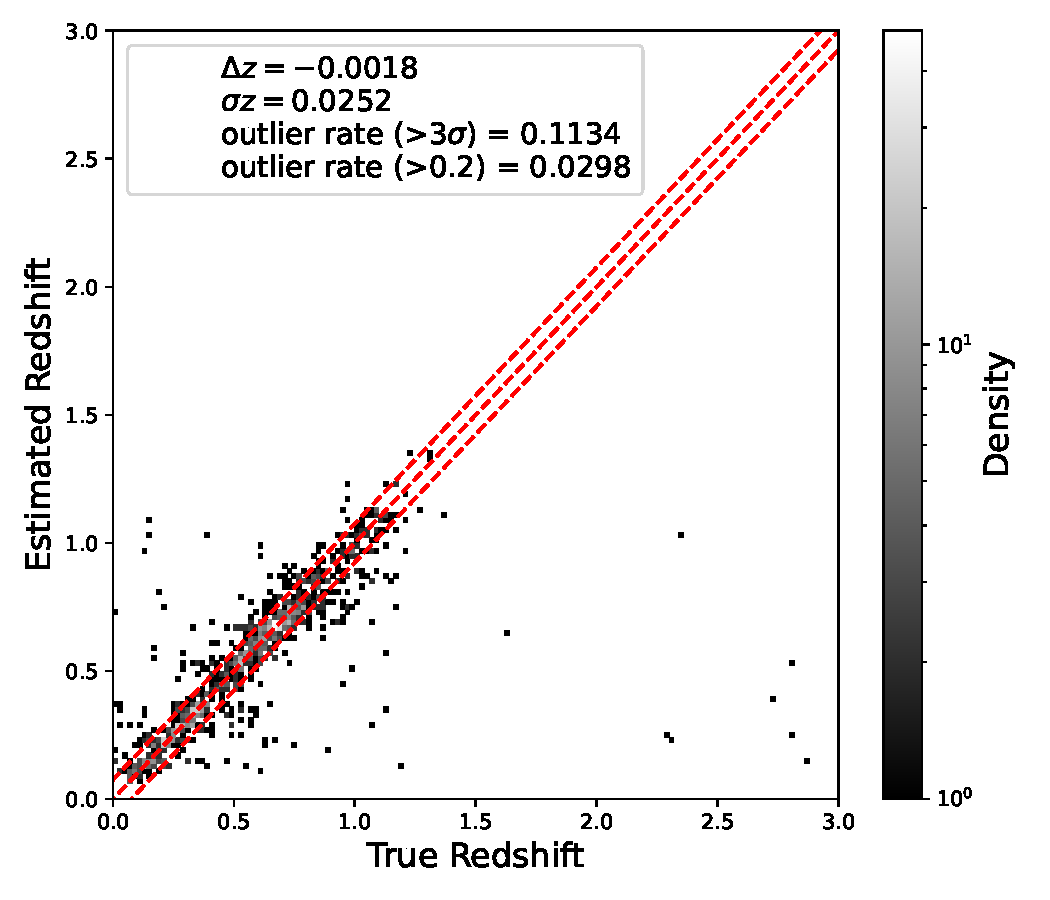
\includegraphics[width=0.45\linewidth]{figures/tpz_scatter_clean.pdf} \\
    \caption{Estimator performance for \code{TPZ} without (left) and with (right) a quality cut of $\sigma_{p(z)} < 0.15$.}
    \label{fig:scatter_quality_cut}
\end{figure*}


\subsubsection{Validation in the \field{SV\_38} field}

We cross-matched our \photoz estimates with the DESI DR1 LSS galaxies (BGS, LRG, and ELG) in the \field{SV\_38} field. This cross-matched catalog can serve as additional validation for our \photoz results.  In Fig.~\ref{fig:sv_validation}, we show the median photometric redshift estimates versus the DESI spectroscopic redshifts all eight tested \photoz algorithms.  Each panel corresponds to a different algorithm, allowing us to visually assess the bias, scatter, and potential outlier behavior across a wide redshift range. Overall, the agreement with DESI DR1 spectroscopic redshifts provides a robust sanity check on the performance of our methods in the early LSST data regime.

\begin{figure*}
\centering
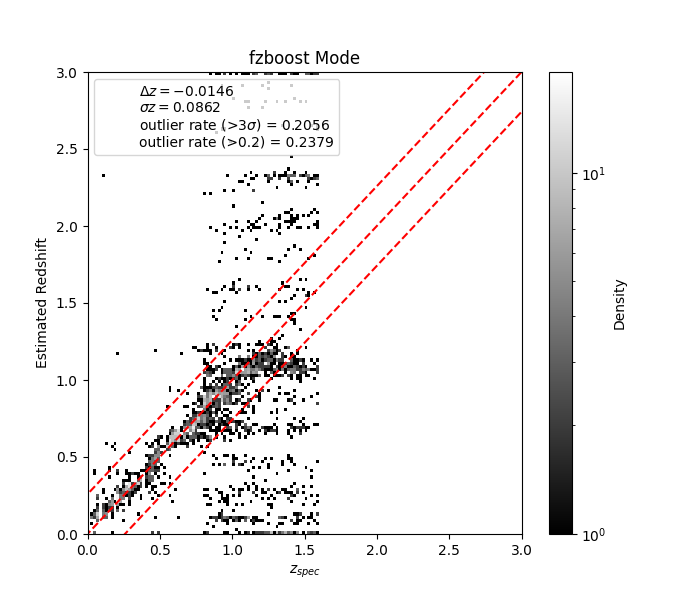
\includegraphics[width=0.32\linewidth]{figures/fzboost_mode_desi.png}
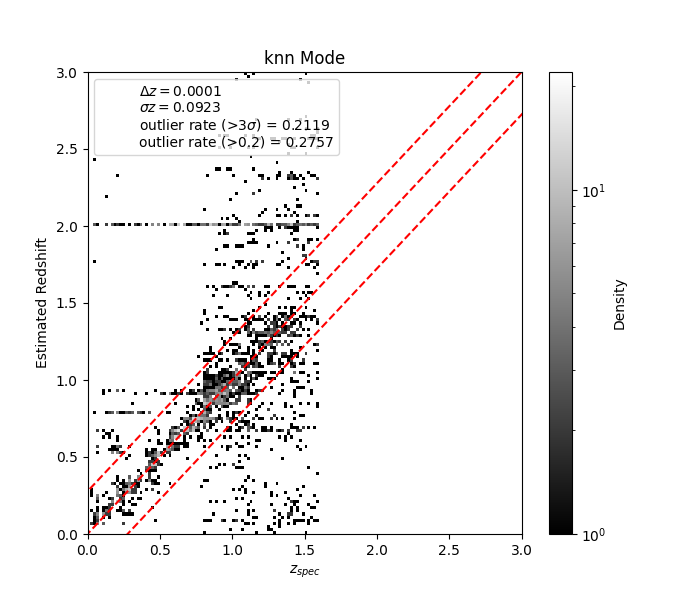
\includegraphics[width=0.32\linewidth]{figures/knn_mode_desi.png}
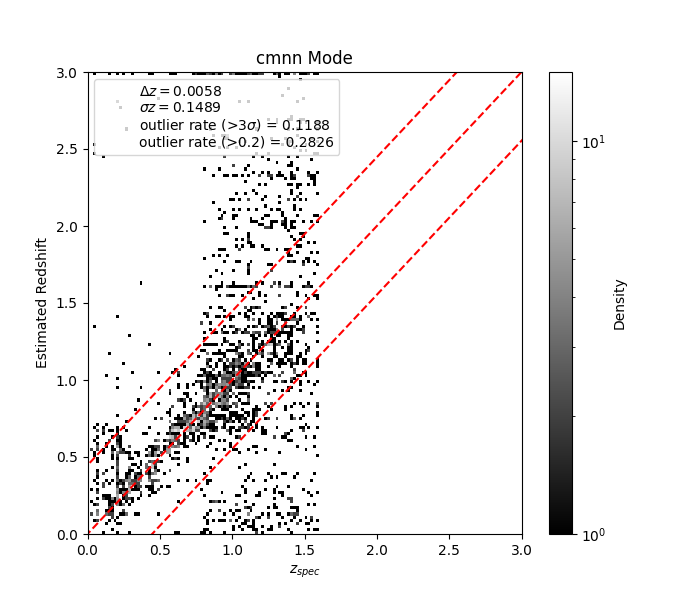
\includegraphics[width=0.32\linewidth]{figures/cmnn_mode_desi.png}
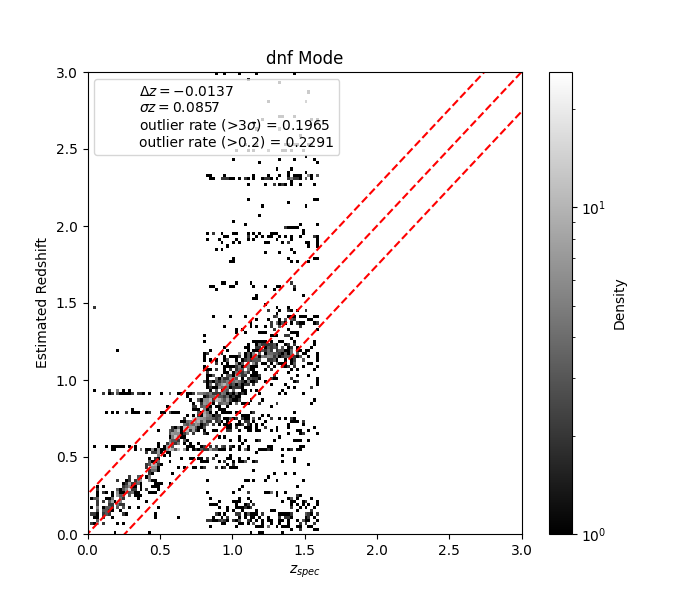
\includegraphics[width=0.32\linewidth]{figures/dnf_mode_desi.png}
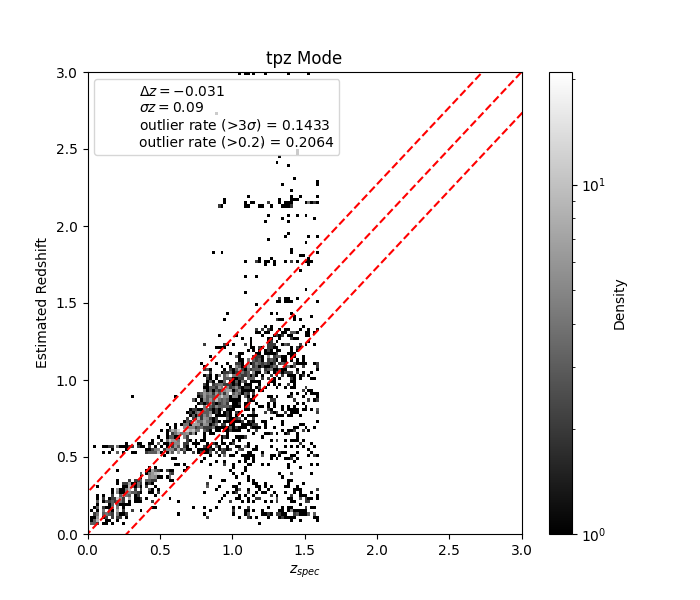
\includegraphics[width=0.32\linewidth]{figures/tpz_mode_desi.png}
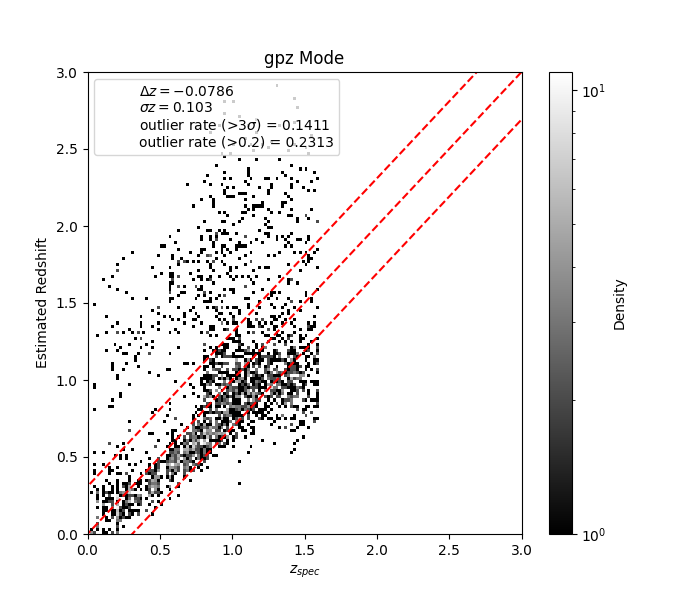
\includegraphics[width=0.32\linewidth]{figures/gpz_mode_desi.png}
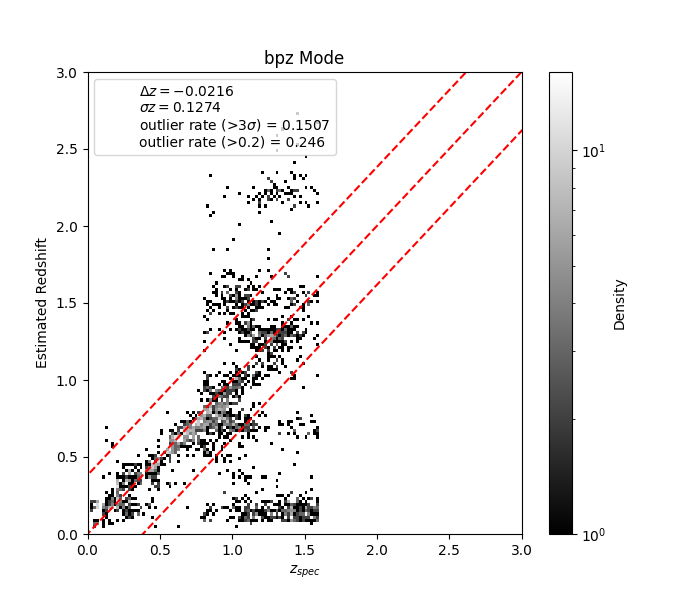
\includegraphics[width=0.32\linewidth]{figures/bpz_mode_desi.png}
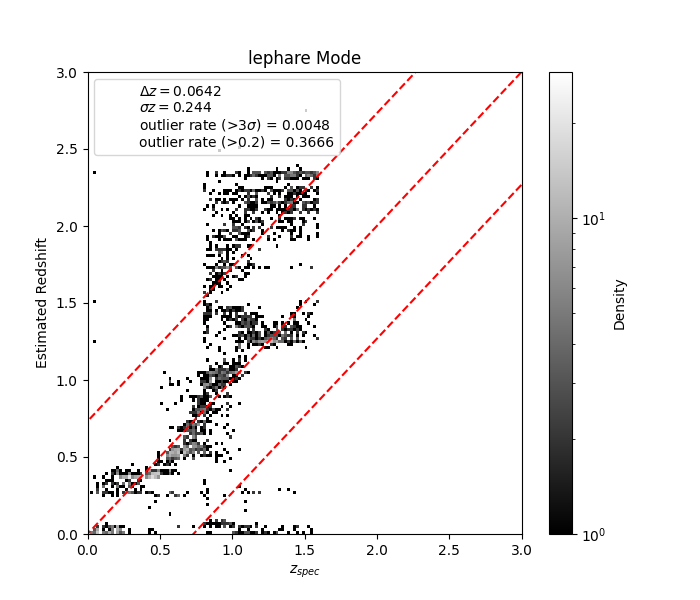
\includegraphics[width=0.32\linewidth]{figures/lephare_mode_desi.png}
\caption{Mode photometric redshift estimates versus DESI DR1 spectroscopic redshifts for galaxies in the \field{SV\_38} cross-matched sample. Each panel shows results from a different \photoz algorithm: FlexZBoost, kNN, CMNN, DNF, TPZ, GPz, BPZ, and LePhare (from left to right, top to bottom). These comparisons provide an external validation of \photoz performance using Large-Scale Structure spectroscopic redshifts samples DESI.}
\label{fig:sv_validation}
\end{figure*}



\subsection{Technical performance}
\label{sec:performance:technical}

Tab.~\ref{tab:tech_perf} shows compute times and file sizes for both the training and estimation phases of the analysis.    The metrics from the training phase were taken from running the algorithm's ``Inform'' stages on USDF on the ``training\_v1'' dataset of ~7,000 objects.    The metrics from the estimation phase were taken from algorithm's ``Inform'' stages on USDF on the ``test\_v1'' datasets of ~2,437 objects.

\begin{table*}
\centering
\begin{tabular}{lllll}
 \hline
  Algorithm name  & \multicolumn{2}{c}{Training}  &  \multicolumn{2}{c}{Estimation} \\
   & Time [s] & Model Size [MB] &  Speed [ms / object] & Data Size [b / object] \\  
 \hline
 \hline
 \multicolumn{5}{c}{Project Supported} \\ 
  \code{BPZ} & $< 5$ & 1 & 1.5-10 & $\sim$ 2400\\
 \code{KNN} & 8 - 30 & 1 & 0.6-1.5 & $\sim$ 240 \\
 \multicolumn{5}{c}{Community Supported} \\   
 \code{CMNN} &  $< 5$ & 1 & 2.4 & 54 \\
 \code{DNF} &  $< 5$ & 2 & 0.6 & $\sim$ 2400 \\
 \code{FlexZBoost}  & 55 - 100 & 35 - 50 & 4-13 & $\sim$ 2400\\
 \code{GPz} & 10 - 15 & 1 & < 0.5 & 32 \\
 \code{LePHARE} & 300 - 600 & 1 & 50 - 180 & $\sim$ 2400 \\
 \code{TPZ} & 5-20 & 7 - 300 & 7 - 120 & $\sim$ 2400 \\
 \hline
\end{tabular}
\caption{
  Algorithm compute times and files sizes.   The algorithms were trained on 7000 objects and evaluated on 2,437 objects.  The variations shown reflect the differences in processing times with different sets of hyper-parameters.
}
\label{tab:tech_perf}
\end{table*}

We note that the technical performance requirements depend heavily on the scientific use case.  For example, in supernova cosmology, the number of objects will be in the 100's of thousands, while for weak-lensing cosmology, it will be in the billions.  Accordingly, these give very different constraints on the required processing speed of the \photoz estimation.  While seconds per object is supportable for supernova cosmology, weak-lensing will require processing times in the milliseconds ($ms$) per object range. 


\section{Limitations and Caveats}
\label{sec:limitations:0}

The \photoz estimates described in this note were done on a best-effort basis by members of the ``Photo-z Science Unit'' and are not official Rubin data products.  As such, the release of the various DP1-related data products comes with a number of caveats.

\begin{itemize}
\item{The size and depth of the training set seriously limits the robustness of the training past a redshift of $z \simeq 1.5$.  See in particular Fig.~\ref{fig:dp_mag_i_v_redshift}.}
\item{In general, \photoz algorithms do not perform well with objects with marginal detections or with non-detections in several bands.  Simply put, the photometric uncertainties in such objects often overwhelms the information that is present and the photometric estimates are very uncertain.  See Fig.~\ref{fig:faint_object_pdf} for an example of the PDF of such an object.   Similarly, see, Fig~\ref{fig:faint_objects} as an illustration of how the accuracy of a \photoz point-estimate degrades significantly for faint objects.}
\item{Taking points (1) and (2) together, we do not advise to use any of the provided DP1 \photoz estimates without applying cuts on the detection significance or the width of the $p(z)$ distribution, or both.}
\item{While we did put some work into optimizing the performance of the various algorithms, this was by no means comprehensive, and we urge caution in drawing any conclusions about the relative merits of the algorithms.}
\item{The training and test sets were drawn from the same set of spectroscopically matched objects.  As such, the training set is fairly representative of the test set.   On the other hand, the full DP1 catalog does not have any spectroscopic selections applied, so the training and test sets will not be representative of the full DP1 data set.}
\end{itemize}

\begin{figure*}
    \centering
    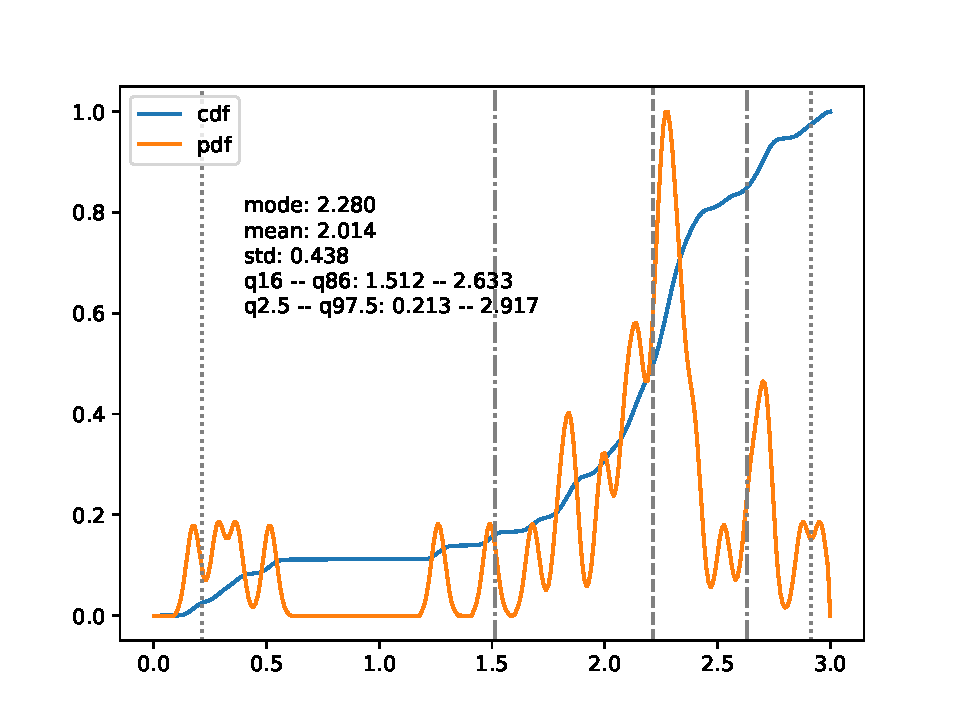
\includegraphics[width=0.45\linewidth]{figures/bad_pdf.pdf}
    \caption{Example of a $p(z)$ distribution for a faint object is not detected in all bands.  (In this case the object was only significantly detected in 'g' and 'r' bands).}
    \label{fig:faint_object_pdf}
\end{figure*}

\begin{figure*}
    \centering
    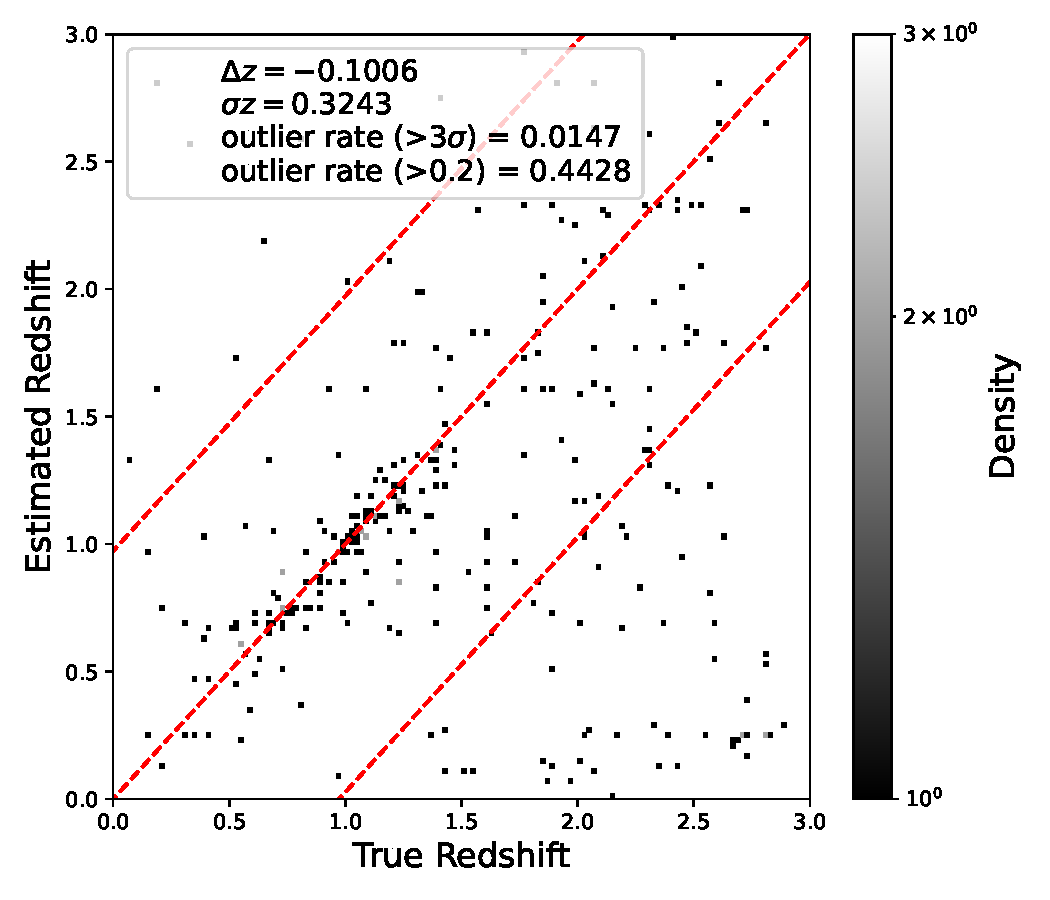
\includegraphics[width=0.45\linewidth]{figures/tpz_scatter_faint.pdf}
    \caption{Point-estimates versus spectroscopic redshifts for all galaxies in the reserved test set with $m_{i} > 23.5$, showing the degradation in estimation performance for faint objects.}
    \label{fig:faint_objects}
\end{figure*}


\section{Summary and Conclusion}
\label{sec:summary:0}

This note describes an initial calculation of photometric redshifts on the Rubin Data Preview 1 dataset using the tools and workflows developed specifically for this purpose by the Photo-z Science Unit.  These early results are very promising, we show that we can successfully match Rubin data with spectroscopic samples in the ECDFS field with deep six-band Rubin coverage to create a reference sample and run our software pipelines to generate a catalog of individual object redshifts consisting of both point 1D redshift PDFs and point estimate redshifts.  We show results for eight \photoz algorithms using a reserve set of redshifts, and see that \photoz performance is in-line with expectations both in terms of our redshift predictions and for compute times.  We also test our estimates against an independent set of redshifts from the \field{SV\_38} field with shallower coverage and imaging in only four of the six Rubin bands.  We describe available data products and anticipated methods to access them.  Overall, this is a very successful initial test of \photoz pipelines.

However, work will continue on several fronts to further optimize the performance of our redshift predictions.  As mentioned earlier in the note, the definition of the true redshift reference sample used to train our algorithms has a large impact on results, being the ``truth'' used to define the flux/color-to-redshift mapping that is inherent to \photoz estimation.  We will work to refine our reference sample definition, which objects to include/exclude based on quality flags, explore the tradeoffs of including grism and many-band \photoz estimates with larger redshift uncertainties in our training sample, and other such effects.  As more and more Rubin data is taken, areal coverage is increasing, including coverage of additional deep calibration fields with existing spec-z datasets.  This will naturally improve \photoz performance.  Expansion of reference redshifts will also enable the development of improved object flagging for identifying which redshifts are trustworthy and those which are likely to be incorrect.

We will also continue to examine the Rubin photometry and evaluate the performance of multiple measurement algorithms.  In this note we used Gaussian Aperture (Gaap) fluxes and magnitudes, as they are expected to produce consistent colors.  We will undertake a thorough exploration of multiple flux measurements (e.~g.~cModel, Sersic, additional Gaap apertures) to test which combinations lead to the best \photoz estimates, as well as combinations like using multiple aperture magnitudes that may contain information on the galaxy light profile that could help to constrain redshift.  As we are still in the engineering and testing phase of the project, there is ongoing work to characterize system performance, and improved understanding of the system will likely lead to better \photoz performance.  For example, there may be some hints that u-band fluxes are overestimated and u-band uncertainties underestimated at faint magnitudes (see the high redshift u-g colors in Fig.~\ref{fig:dp_color_v_redshift} and figures in~\citet{RTN:095}).  DP1 data was obtained using ComCam, while future data releases will use LSSTCam, and thus performance for DP2 and beyond may be shaped by slight differences between the two instruments.  

In this analysis, while there was some optimization of code-specific parameters for the individual estimators, e.~g.~the number of neighbors used for \code{KNN}, the number of trees used for \code{TPZ}, it was not comprehensive.  In addition, the optimal values will likely change slightly as we refine both our spectroscopic reference sample and our photometric inputs.  A thorough exploration of the code parameters will happen as we converge on our final photometric and spectroscopic setup.

As stated in the introduction, we expect feedback from science users as they explore the data and discover issues that we have not anticipated, and that we will incorporate that feedback in future work.

Key takeaway: while very promising, these results are far from final, there is ongoing work to optimize \photoz performance.  We have plans in place and will continue to refine as new data arrives, and these plans should lead to improved redshift performance. 

\pagebreak




%  LocalWords:  citep photozs photozs citep photoz photoz texttt griz
%  LocalWords:  subsubsection texttt _gaap1p0FluxErr texttt _psfFlux
%  LocalWords:  _ecdfs ugrizy _psfFluxErr hline fig:dp_mags linewidth
%  LocalWords:  fig:dp_mag_i_v_redshift fig:dp_color_v_redshift grism
%  LocalWords:  fig:dp_color_v_color includegraphics citet 2dflens
%  LocalWords:  colless2001 huchra2012 momcheva2016 kodra2023 Abell
%  LocalWords:  deugenio2025 helou1991 garilli2021 lefevre2013 textit
%  LocalWords:  approx0.25 rail-bpz rail-sklearn rail-cmnn rail-dnf
%  LocalWords:  FlexZBoost GPz Almosallam:2016 rail-lephare rail-tpz
%  LocalWords:  Lephare _bpz Ilbert:09 _bpz _bpz _pz _optimze knn bpz
%  LocalWords:  rightarrow rightarrow knn bpz textbf textbf textbf
%  LocalWords:  Sersic



\appendix

% Include all the relevant bib files.
% https://lsst-texmf.lsst.io/lsstdoc.html#bibliographies
\section{References} \label{sec:bib}
\renewcommand{\refname}{} % Suppress default Bibliography section
\bibliography{local,lsst,lsst-dm,refs_ads,refs,books}

% Make sure lsst-texmf/bin/generateAcronyms.py is in your path
\section{Acronyms} \label{sec:acronyms}
\addtocounter{table}{-1}
\begin{longtable}{p{0.145\textwidth}p{0.8\textwidth}}\hline
\textbf{Acronym} & \textbf{Description}  \\\hline

DESI & Dark Energy Spectroscopic Instrument \\\hline
DP1 & Data Preview 1 \\\hline
DR1 & Data Release 1 \\\hline
ECDFS & Extended Chandra Deep Field-South Survey \\\hline
LSST & Legacy Survey of Space and Time (formerly Large Synoptic Survey Telescope) \\\hline
SE & System Engineering \\\hline
photo-z & photometric redshift \\\hline
\end{longtable}

% If you want glossary uncomment below -- comment out the two lines above
%\printglossaries





\end{document}
